%!TEX root = main.tex



%We are ready to define prioritized streaming string transducers. 
%In the definition, 
%
%The special symbol $\nullchar$ is introduced to capture the situation that $\extract_{i,e}(x)$ returns $\nullchar$, i.e. $x \in \Lang(e)$ but the $i$-th capturing group of $e$ is not matched.
%

%\paragraph{Semantics}
 
%We now define the formal semantics of $\regexp$. Traditionally, regular expressions are interpreted as a regular language, i.e., a set of strings, which can be defined inductively in a rather straightforward way. In our case when the regular expression is used in string constraints arisen from analysis of programming language such as JavaScript, %owing to the introduction of greedy/lazy semantics,  
%what we need is not only the language denoted by the regular expression, but also the intermediate result when parsing a string against the given regular expression. This is especially the case when the capturing group is involved. As a result, we need a more operational (as opposed traditional denotational) account of the semantics for regular expression. To this end, we harness an extension of finite-state automata with priorities, which \emph{defines} how a string is accepted by the given regular expression. We start with the standard finite-state automaton.  



%We now define the formal semantics of {\regexp}. 
%Note that traditionally regular expressions are interpreted as a regular language, i.e., a set of strings, which can be defined inductively in a rather straightforward way. 
%In our case when the regular expression is used in string constraints arisen from analysis of programming language such as JavaScript, %owing to the introduction of greedy/lazy semantics,  
%what we need is not only the language denoted by the regular expression, but also the intermediate result when parsing a string against the given regular expression. This is especially the case when the capturing group is involved. As a result, 
%
%Here we present a more operational (as opposed traditional denotational) account of the semantics by constructing  PSSTs out of regular expressions (cf.\ Section~\ref{sect:regextopsst}). 
%
 
We now define the formal semantics of {\regexp}. Traditionally they are interpreted as a regular language which can be defined inductively. 
In our case, where {\regexp} are mainly used in string functions, %arisen from analysis of programming language such as JavaScript, %owing to the introduction of greedy/lazy semantics,  
what matters is %not only the language denoted by the regular expression, but also 
the intermediate result when parsing a string against the given {\regexp}. %This is especially the case when the capturing group is involved. 
As a result, we shall present an operational (as opposed to traditional denotational) account of the \regexp-string matching by constructing {\PSST}s out of regular expressions. 


%, which  is defined by recursively constructing {\PSST}s out of regular expressions.
Note that in \cite{BDM14,BM17}, a construction from {\regexp} to prioritized finite transducers (PFT) was given. The construction therein is a variant of the classical Thompson construction from regular expressions to nondeterministic finite automata \cite{Thompson68}. In particular, the size of the constructed PFT is linear in the size of the given {\regexp}. One may be tempted to think that the construction in \cite{BDM14,BM17} can be easily adapted to construct {\PSST}s out of regular expressions. 
%
Nevertheless, the construction in \cite{BDM14,BM17} does \emph{not} work for so called \emph{problematic regular expressions}, i.e.,  those regular expressions that contain the subexpressions $e^*$ or $e^{*?}$ with $\varepsilon \in \Lang(e)$. Moreover, the construction therein did not consider the repetition operators $[e_1^{\{m_1,m_2\}}]$ or $[e_1^{\{m_1,m_2\}?}]$. 
%Finally, the construction therein was not validated against the actual semantics of regex-string matching in programming languages. 
%
Our construction, which is considerably different from that in \cite{BDM14,BM17}, works for arbitrary regular expressions. In particular, the size of the constructed {\PSST} can be \emph{exponential} in the size of the given regular expression in the worst case. Moreover, we validate by extensive experiments that our construction is consistent with the actual \regexp-string matching in JavaScript. %The size of the constructed {\PSST} can be \emph{exponential} in the size of the given regular expression in the worst case.

%\subsection{Semantics of \regexp[\sf CG]}
%In this section, we give one of the many semantics of \regexp[\sf CG], which we will utilize for $\replaceall$.
%For two indexed $\regexp$s $e$ and $e'$, we say $e'$ is a \emph{subexpression} of $e$,
%if one of the following conditions holds: 1) $e'=e$, 2) $e = [e_1 \cdot e_2]$ or $[e_1 + e_2]$, and $e'$ is a subexpression of $e_1$ or $e_2$, 3) $e = [e^?], [e^{??}], [e_1^{\ast}]$, $[e_1^{+}]$, $[e_1^{\ast?}]$, $[e_1^{+?}]$, $e_1^{\{m_1, m_2\}}$, $e_1^{\{m_1, m_2\}?}$ or $(_n e_1)_n$, and $e'$ is a subexpression of $e_1$. We use $S(e)$ to denote the set of all subexpressions of $e$. %\tl{is there a difference between $[e_1\cdot e_2]$ and $e_1 e_2$?}
%
% 
%By a mutual induction on $|w|$ and $|e|$, we can show that $|\cM_{w}(e)|$, the size of $\cM_{w}(e)$, is at most $|w||e|$.  

%\begin{example}\label{exmp-regex-match-tree}
%	Let $w= 0250$ and $e = [[([\Gamma^+])\concat .?] \concat ([\Gamma^*])]$ where $\Gamma = \{0,1,\cdots,9\}$. Note that $e$ is essentially {\tt decimalReg} in the motivating example. Then $\cM_{w}(e) = \{T_1,T_2,T_3, T_4\}$ as illustrated in Figure~\ref{fig-regex-semantics-decimal}(i), (ii), (iii), and (iv), where the match trees rooted at $(0, \Gamma)$, $(2, \Gamma)$, and $(5, \Gamma)$ are omitted. % to avoid tediousness.
%	\begin{figure}[htb]
%		\centering
%		%\rule{\linewidth}{0cm}
%		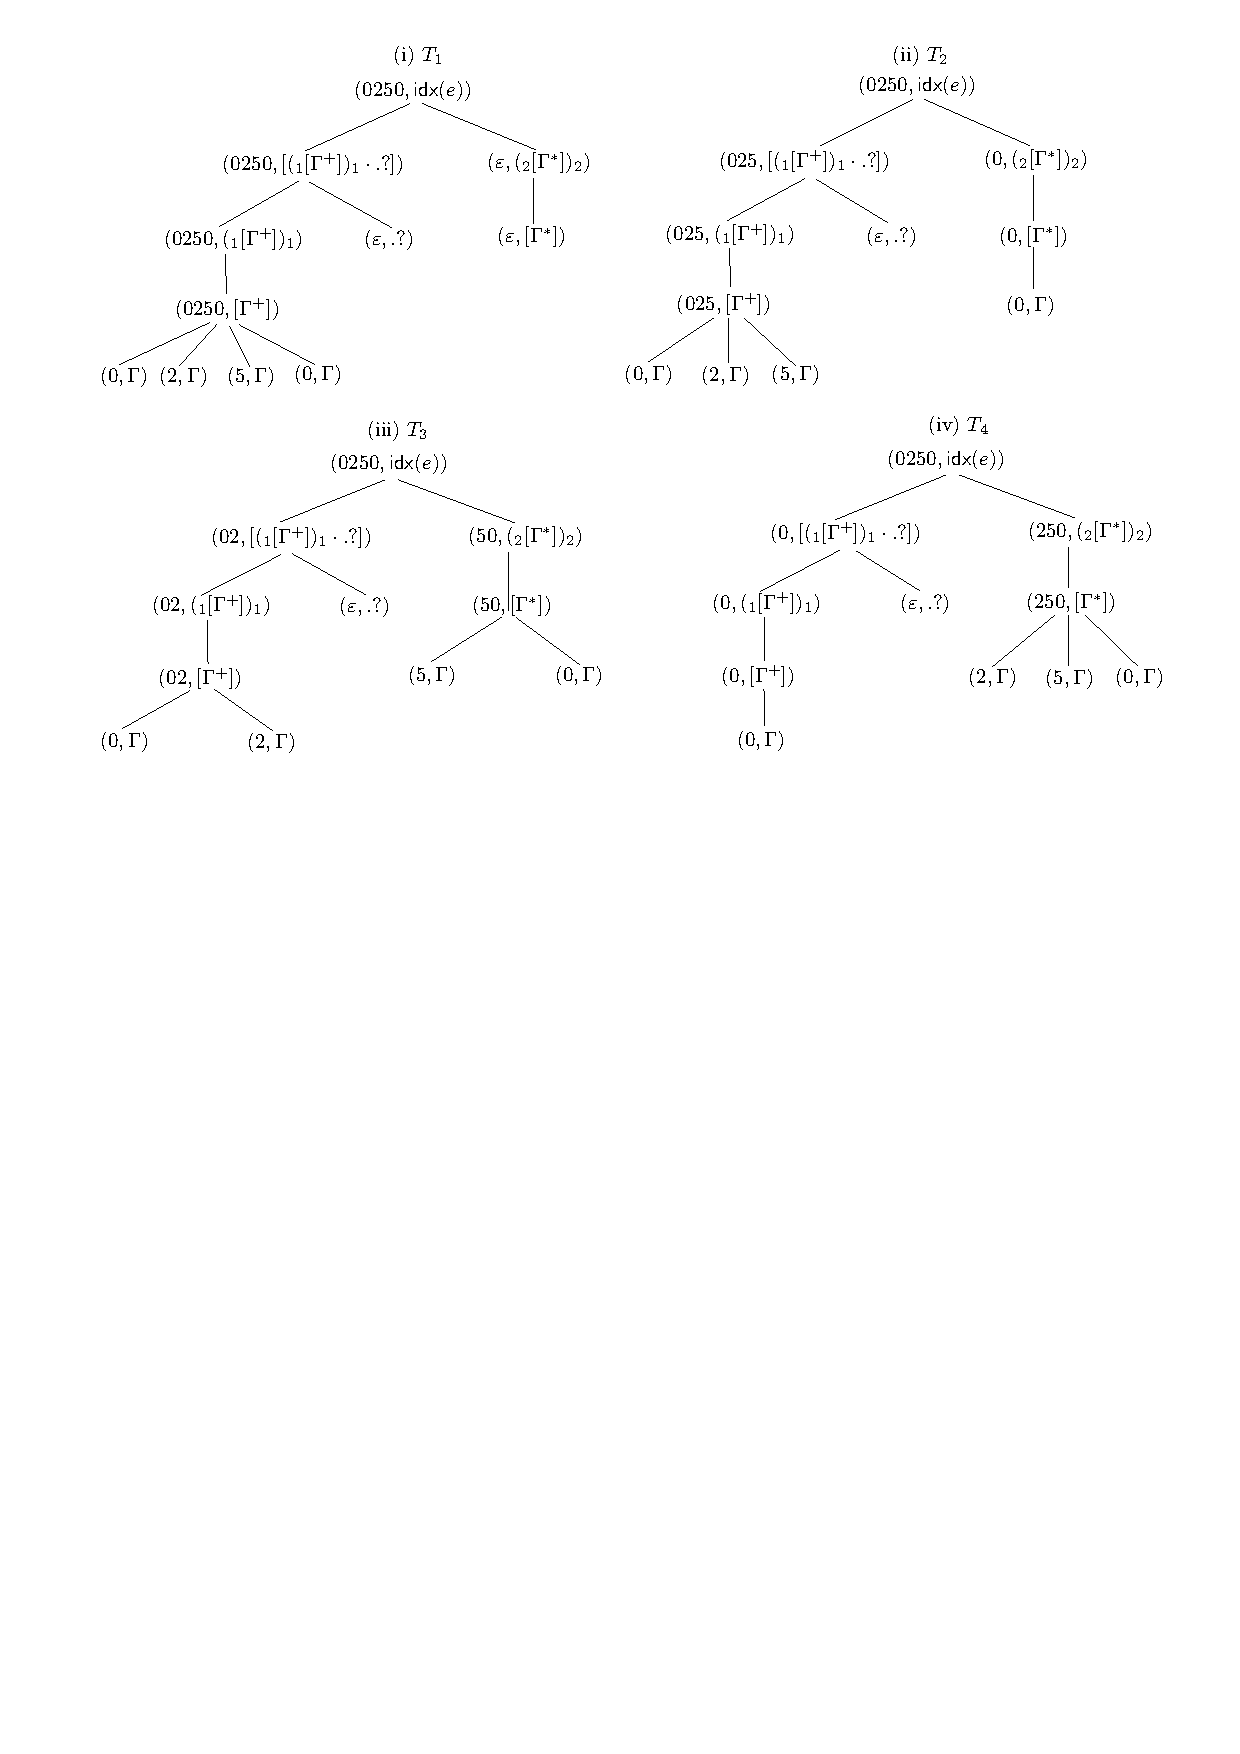
\includegraphics[width=1\textwidth]{regex-semantics-decimal.pdf}
%		\caption{Match trees of $e=[[([\Gamma^+])\concat .?] \concat ([\Gamma^*])]$ to $w= 0250$}
%		\label{fig-regex-semantics-decimal}
%		
%	\end{figure}
%	%\Blindtext
%\end{example}

 
 
%
%\begin{example}\label{exmp-regex-semantics}
%	Let us continue Example~\ref{exmp-regex-match-tree}.  In Fig.~\ref{fig-regex-semantics-decimal}, we have $(T_1)_{(0250, [\Gamma^+])} >_{(w, \idxexp(e))} (T_2)_{(025, [\Gamma^+])}$, since $(0, \Gamma)(2, \Gamma)(5,\Gamma)$ is a proper prefix of $(0, \Gamma)(2, \Gamma)(5,\Gamma)(0, \Gamma)$. Then we deduce that $(T_1)_{(0250, (_1[\Gamma^+])_1)} >_{(w, \idxexp(e))} (T_2)_{(025, (_1[\Gamma^+])_1)}$. Consequently, $(T_1)_{(0250, [(_1[\Gamma^+])_1 \concat .?])} >_{(w, \idxexp(e))} (T_2)_{(025,  [(_1[\Gamma^+])_1 \concat .?])}$ and $T_1 >_{(w, \idxexp(e))} T_2$. Similarly, we have $T_2 >_{(w, \idxexp(e))} T_3$ and $T_3 >_{(w, \idxexp(e))} T_4$. Therefore, $T_1$ is the accepting match of $e$ to $w$, where the first and second capturing group of $e$ are matched to $0250$  and $\varepsilon$ respectively. 
%	%\Blindtext
%\end{example}

%\begin{remark}
%	Our semantics of $\regexp$ follows the 11th Edition of the ECMAScript specification (ES11 for short) \cite{ECMAScript11}, with a focus on the non-commutative union, the greedy/lazy semantics of Kleene star/plus, as well as capturing groups and backreferences.
%	In comparison, POSIX regular expressions require the leftmost and longest match of regular expressions, which we leave as future work.
%\end{remark}


% some examples

%  e = b(a*)a*
%  
%  e' = b(a*?)a*

%\begin{figure}[ht]
%\centering
%\rule{\linewidth}{0cm}
%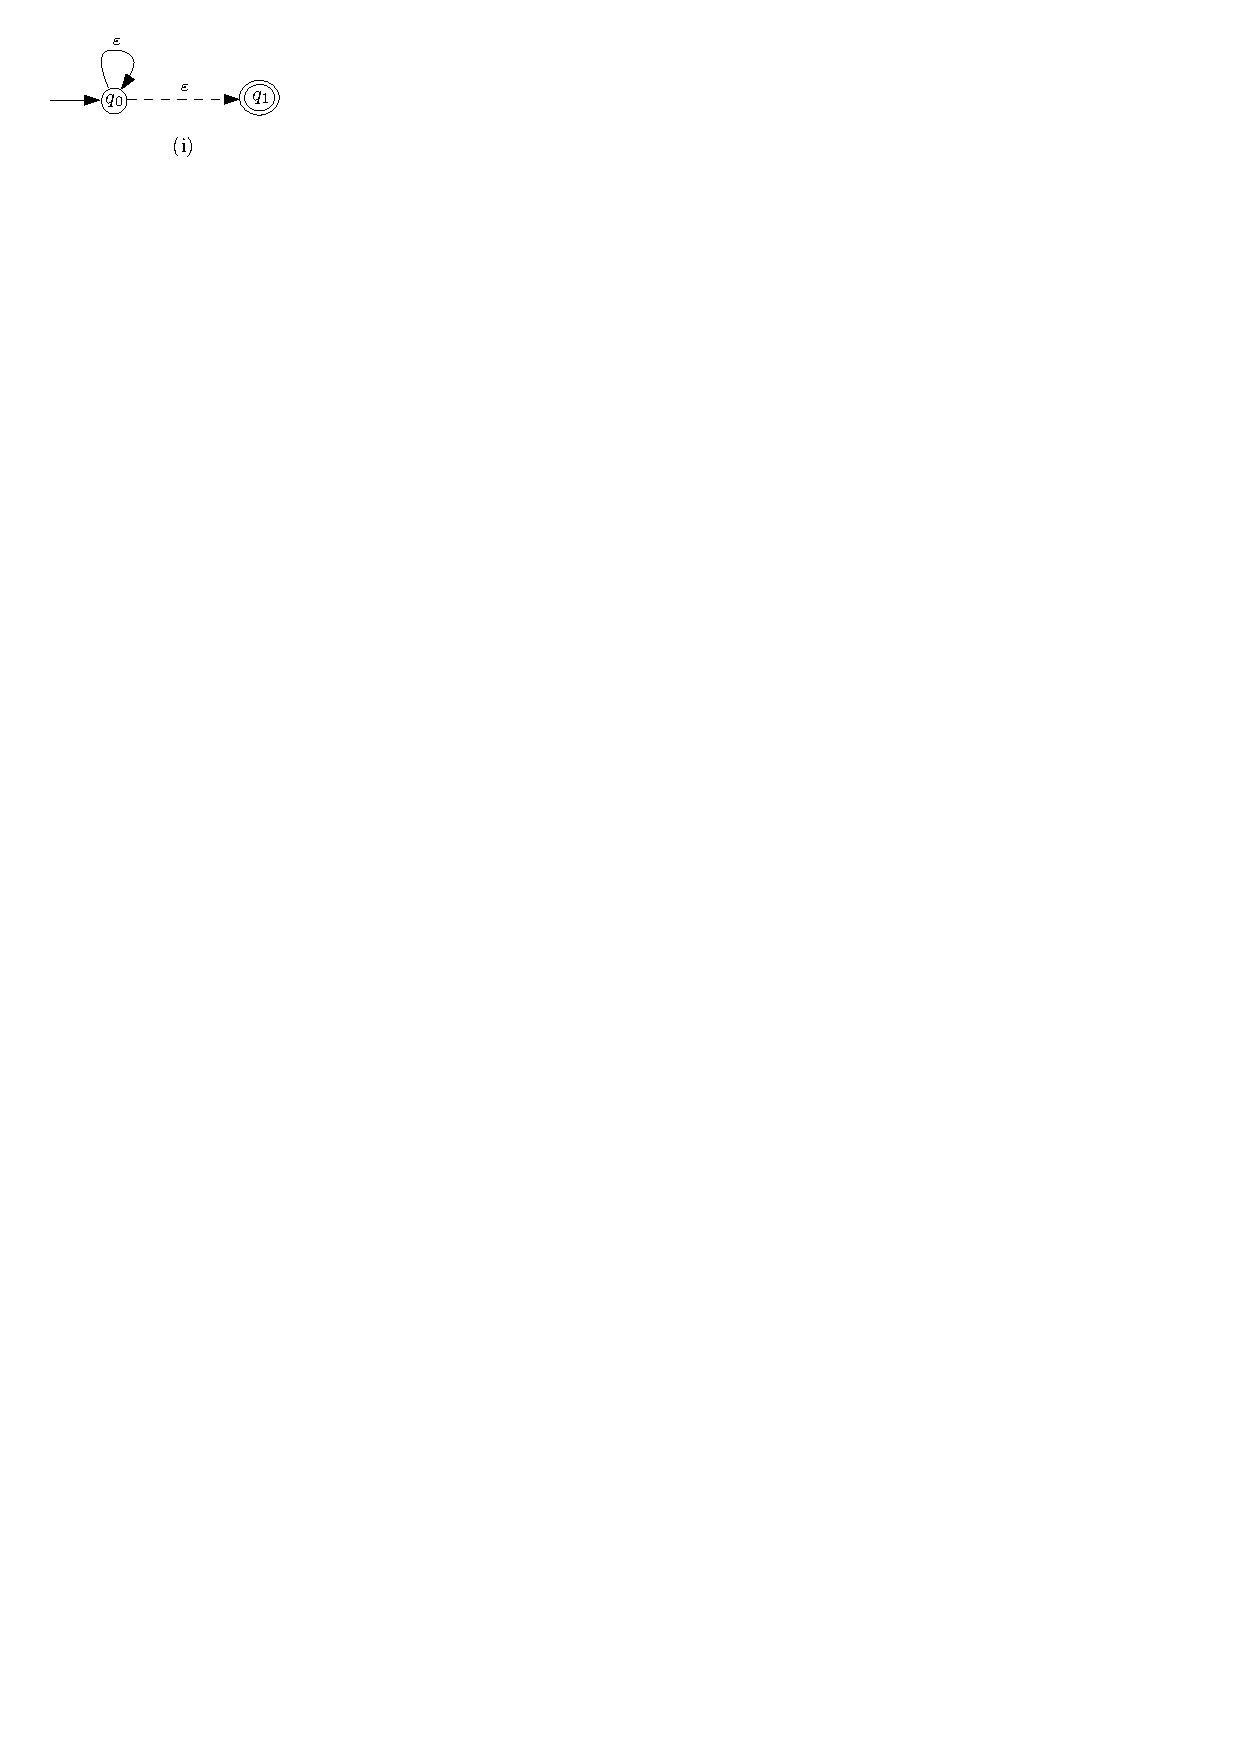
\includegraphics[scale=0.8]{pfa-epsilon-star.pdf}
%\caption{The PFA for $\varepsilon^\ast$}
%\label{fig-pfa-epsilon-star}
%\end{figure}



%%%%%%%%%%%%%%%%%%%%%%%%%%%%%%%%%%%%%%%%%%%%%%%%%%%%%%%%%%%%%%%%%%%%%%%%%%%%%%%%%%%%%%%%%%%%

%We can adapt the PFA construction in \cite{BDM14}, which in turn is a variant of the standard Thompson construction \cite{Thompson68}, and show the following result. 

%\begin{proposition}\label{prop-rwre-to-pfa}

%We associate with each regular expression $e$ a PFA $\cA_e$ and define the semantics of $e$ as the language accepted by $\cA_e$. As expected, the PFA $\cA_e$ is constructed inductively. 

The main idea of the construction is to split the set of final states, $F$, into two disjoint subsets $F_1$ and $F_2$, with the intention that $F_1$ and $F_2$ are responsible for accepting the empty string resp. non-empty strings. Note here for technical convenience, we assume that $F$ in a {\PSST} is a set of final states, instead of an output function. Therefore, the {\PSST}s constructed in the sequel are of the form $(Q, \Sigma, X, \delta, \tau, E, q_0, (F_1, F_2))$. 
%
Furthermore, to deal with the situation that some capturing group may not be matched to any string and its value is undefined, we introduce a special symbol $\nullchar$ %for denoting this situation 
and assume that the initial values of all the string variables are $\nullchar$. %To avoid the tediousness, 
For simplicity, in the definition of a {\PSST}, if $\delta(q, a, q') = ()$ or $\tau(q, \varepsilon, q') = ((); ())$,  they will not be stated explicitly. Moreover, we will omit all the assignments $E(q, a, q')(x)$ such that $E(q, a, q')(x) = x$.
%By default, all the PSSTs from now on satisfy these assumptions. 

For {\PSST}s of the form $(Q, \Sigma, X, \delta, \tau, E, q_0, (F_1, F_2))$, we introduce a notation to be used in the construction, namely, the concatenation of two {\PSST}s. 

\begin{definition}[Concatenation of two PSSTs]\label{def-psstconcat}
For $i \in \{1,2\}$, let $\cT_i = (Q_i, \Sigma, X_i, \delta_i, \tau_i, E_i, q_{i,0}, (F_{i,1}, F_{i,2}))$ be a PSST. Then the \emph{concatenation} of $\cT_1$ and $\cT_2$, denoted by $\cT_1 \concat \cT_2$, is defined as follows (see Figure~\ref{fig-psstconcat}): 
Let  
$\cT'_{2} = (Q'_{2}, \Sigma, X_{2}, \delta'_{2}, \tau'_{2}, E_{2}', q'_{2,0}, (F'_{2, 1}, F'_{2,2}))$ be a fresh copy of $\cT_{2}$, but with the string variables of $\cT_{2}$ kept unchanged. 
Then 
%
\[\cT = ( Q_{1} \cup Q_{2} \cup Q'_{2}, \Sigma, X_1 \cup X_2, \delta, \tau, q_{1,0}, (F_{2,1}, F_{2,2} \cup F'_{2,1} \cup F'_{2,2}))\] 
where 
	\begin{itemize}
	\item $\delta$ comprises the transitions in $\delta_1$, $\delta_2$, and $\delta'_2$,
%	\begin{itemize}
%	\item for every $a \in \Sigma$, $\delta_e(q_{e,0}, a) = ()$,
	%
%	 \item for every $i \in \{1,2\}$, $q \in Q_{e_i}$ and $a \in \Sigma$, $\delta_e(q, a) = \delta_{e_i}(q, a)$,
%
%	\item for every $q' \in Q'_{e_2}$ and $a \in \Sigma$, $\delta_e(q', a) = \delta'_{e_2}(q',a)$, 
%	 \end{itemize}
			%
	\item $\tau$ comprises the transitions in $\tau_1$, $\tau_2$, $\tau'_2$, and the following transitions,
	\begin{itemize}
%	\item for every $q \in Q_{1} \setminus (F_{1,1} \cup F_{1,2})$, $\tau(q) = \tau_{1}(q)$, 
%
	\item for every $f_{1,1} \in F_{1,1}$, $\tau(f_{1,1}) = ((q_{2,0}); ())$, 
%
	\item for every $f_{1,2} \in F_{1,2}$, $\tau(f_{1,2}) = ((q'_{2,0}), ())$,
	\end{itemize}
	%
	\item $E$ inherits all the assignments in $E_1$, $E_2$, and $E'_2$, and includes the following assignments:  for every $f_{1,1} \in F_{1,1}$, $f_{1,2} \in F_{1,2}$, and $x' \in X_2$, $E(f_{1,1}, \varepsilon, q_{2,0})(x') = E(f_{1,2}, \varepsilon, q'_{2,0})(x')= \nullchar$. (Intuitively, the values of all the variables in $X_2$ are reset when entering $\cT_2$ and $\cT'_2$.)
  \end{itemize}
% Fig.~\ref{fig-reg2pfa-2} depicts the construction. 
		\begin{figure}[tb]
			\vspace{-2mm}
			\centering
			%\rule{\linewidth}{0cm}
			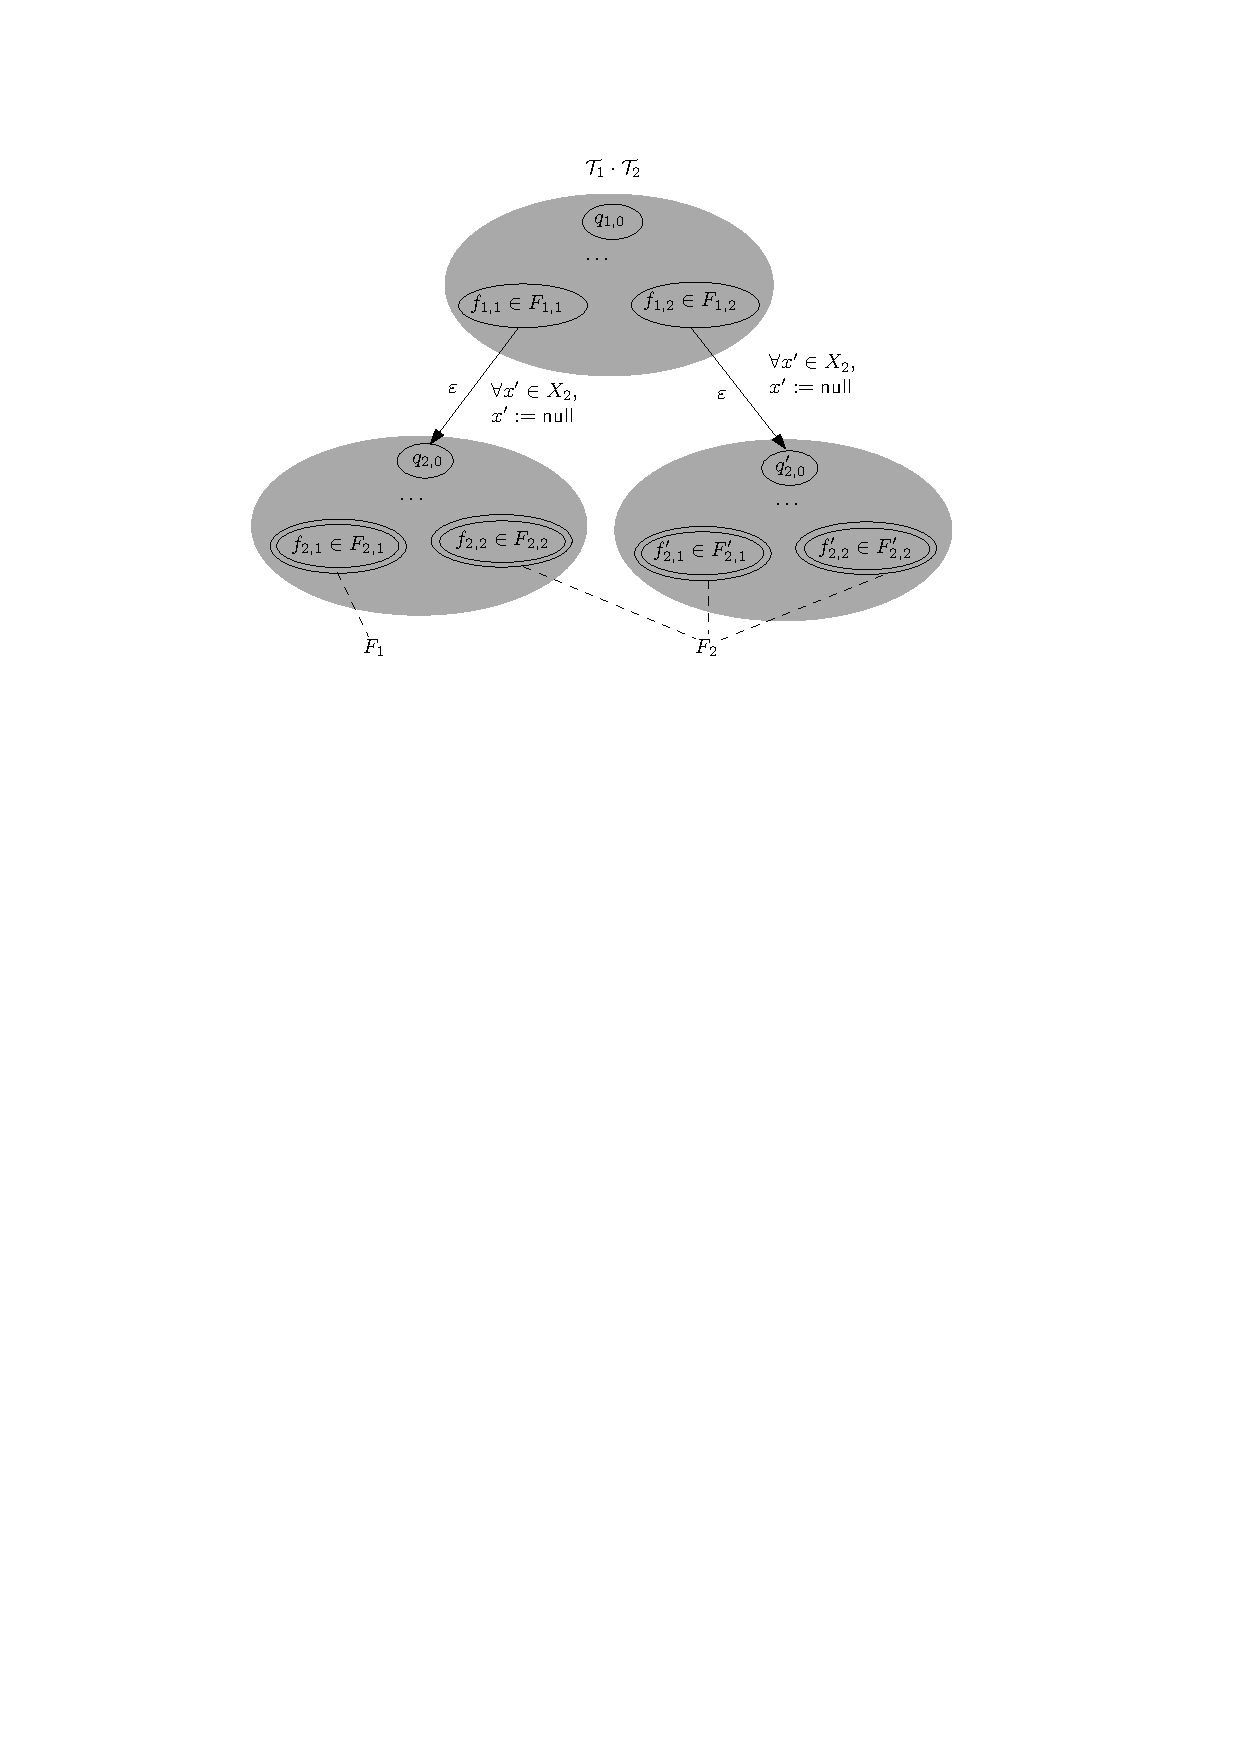
\includegraphics[width = 0.5\textwidth]{psstconcat.pdf}
			\caption{$\cT_1\concat \cT_2$: Concatenation of $\cT_1$ and $\cT_2$}
			\label{fig-psstconcat}
			\vspace{-4mm}
		\end{figure}  
\end{definition}
Note that in the above definition, it is possible that $X_1 \cap X_2 \neq \emptyset$. We   remark that if $F_{1,1} = \emptyset$ or $F_{2,1} = \emptyset$, then \emph{one copy} of $\cT_2$, instead of two copies, is sufficient for the concatenation.

We shall recursively construct a {\PSST} $\cT_e$ for each {\pcre} $e$, such that the initial state has no incoming transitions and each of its final states has no outgoing transitions. Moreover, all the transitions out of the initial state are $\varepsilon$-transitions. 
%
%For convenience, we assign a unique index for each subexpression in a {\pcre}. 
%Let us use $\idx_e$ to denote the index function associated with a {\pcre} $e$. 
We assume that in $\cT_e$, a string variable $x_{e'}$ is introduced for each subexpression $e'$ of $e$. 

Note that the construction is technical and below we only select to present some representative cases. The other cases are relegated to Appendix~\ref{app:reg2psst}.
%Moreover, a special symbol $\nullchar$ is introduced to deal with the situation that a subexpression $e'$ is not matched. If this happens, then the value of $e'$ is undefined and $\nullchar$ is assigned to $x_{e'}$. 
%Let $X_e$ denote the set of string variables introduced for $e$.

%%%%%%%%%%%%%%%%% move to appendix %%%%%%%%%%%%%%%%%%%%%%%%%%%%%%%%%%%

%\paragraph{Case $e =\emptyset$ (see Figure~\ref{fig-reg2pfa-0})} $\cT_\emptyset = (\{q_{\emptyset, 0}\}, \Sigma, \{x_{\emptyset}\}, \delta_\emptyset, \tau_\emptyset, E_\emptyset, q_{\emptyset, 0}, (\emptyset, \emptyset))$, where there are no transitions out of $q_{\emptyset,0}$, namely, $\delta_\emptyset(q_{\emptyset, 0}, a) = ()$ for every $a \in \Sigma$, $\tau_\emptyset(q_{\emptyset, 0}) = ((); ())$, and $E_\emptyset$ is vacuous here.
%%$\delta_\emptyset(q_{\emptyset, 0}, a) = ()$ for every $a \in \Sigma$, $\tau_\emptyset(q_{\emptyset, 0}) = ((); ())$, and $E_\emptyset$ is vacuous here. 
%
%
%\paragraph{Case $e = \varepsilon$ (see Figure~\ref{fig-reg2pfa-0})} $\cT_\varepsilon = (\{q_{\varepsilon, 0}, f_{\varepsilon,0}\}, \Sigma, \{x_\varepsilon\}, \delta_\varepsilon, \tau_\varepsilon, E_\varepsilon, q_{\varepsilon,0}, (\{f_{\varepsilon,0}\}, \emptyset))$, 
%%
%where 
%%$\delta_\varepsilon(q_{\varepsilon,0}, a) = \delta_\varepsilon(f_{\varepsilon,0}, a) = ()$ for every $a \in \Sigma$, 
%$\tau_\varepsilon(q_{\varepsilon,0}) = ((f_{\varepsilon,0}); ())$, %for each transition $(q, a, q')$, 
%and $E_\varepsilon(q_{\varepsilon,0}, \varepsilon, f_{\varepsilon,0})(x) = \varepsilon$. Note $F_2 = \emptyset$ here. 
%		
%\paragraph{Case $e = a$ (see Figure~\ref{fig-reg2pfa-0})} $\cT_a = (\{q_{a,0}, q_{a,1}, f_{a,0}\}, \Sigma, \{x_a\}, \delta_a, \tau_a, E_a, q_{a,0}, (\emptyset, \{f_{a,0}\}))$, where 
%%$\delta_a(q_{a,0}, b) = ()$ for every $b \in \Sigma$, 
%$\tau_a(q_{a,0}) = ((q_{a,1}); ())$, 
%%
%$\delta_a(q_{a,1}, a) = (f_{a,0})$, 
%%$\delta_a(q_{a,1}, b) = ()$ for every $b \in \Sigma \setminus \{a\}$,
%%
%%$\tau_a(q_{a,1}) = ((); ())$, and $\tau_a(f_{a,0}) = ((); ())$, 
%%
%$E_a(q_{a,0}, \varepsilon, q_{a,1})(x_a) = \varepsilon$, and $E_a(q_{a,1}, a, f_{a,0})(x_a) =x_aa$. Note $F_1 = \emptyset$ here. 
%%		
%\begin{figure}[ht]
%			\centering
%			%\rule{\linewidth}{0cm}
%			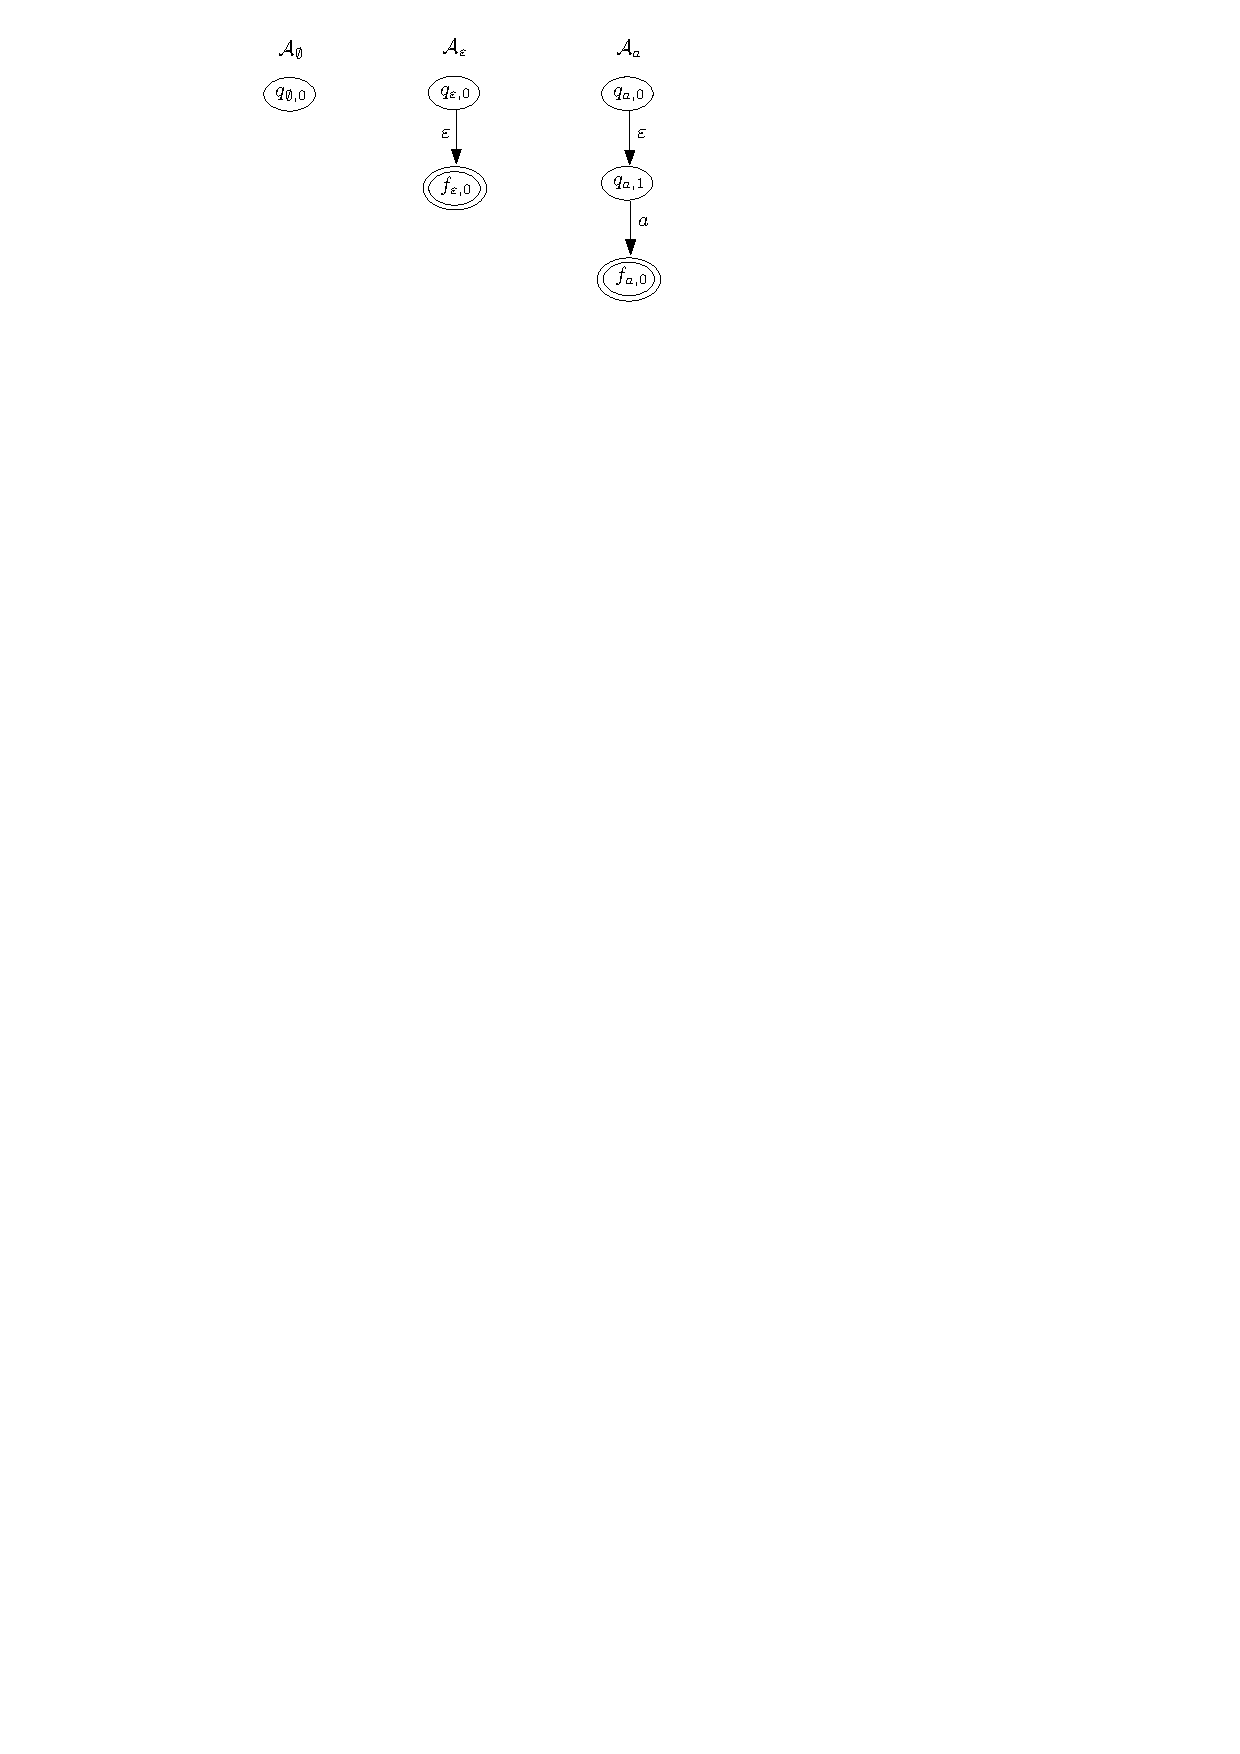
\includegraphics[width = 0.4\textwidth]{reg2pfa-0.pdf}
%			\caption{The PSST $\cT_{\emptyset}$, $\cT_{\varepsilon}$, and $\cT_{a}$ }
%			\label{fig-reg2pfa-0}
%\end{figure}  
%%%%%%%%%%%%%%%%% move to appendix %%%%%%%%%%%%%%%%%%%%%%%%%%%%%%%%%%%
%%%%%%%%%%%%%%%%%%%%%%%%%%%%%%%%%%%%%%%%%%%%%%%%%%%%%%%%%%%%%%%%%%%%%%%%%%%%%%%%%%%%%%%%%%%%%%%%%%%%

		
\paragraph{Case $e = (e_1)$} $\cT_e$ is adapted from $\cT_{e_1} = (Q_{e_1}, \Sigma, X_{e_1}, \delta_{e_1}, \tau_{e_1}, E_{e_1},  q_{e_1,0}, (F_{e_1,1}, F_{e_1,2}))$ by adding the string variable $x_e$ and the assignments for $x_e$, that is, $X_e = X_{e_1} \cup \{x_e\}$ and for each transition $(q, a, q')$ in $\cT_{e_1} $ with $a \in \Sigma^\varepsilon$, we have $E_e(q, a, q')(x_e) = E_{e_1}(q, a, q')(x_{e_1})$. 
		

\paragraph{Case $e = [e_1 + e_2]$ (see Figure~\ref{fig-reg2pfa-1})} For $i \in \{1, 2\}$, let  
$\cT_{e_i} = (Q_{e_i}, \Sigma, X_{e_i}, \delta_{e_i}, \tau_{e_i}, E_{e_i},  q_{e_i,0}, (F_{e_i,1}, F_{e_i,2}))$. Moreover, let us assume that $X_{e_1} \cap X_{e_2} = \emptyset$.
%$\cT_{e_2} = (Q_{e_2}, \Sigma, X_{e_2}, \delta_{e_2}, \tau_{e_2}, E_{e_2}, q_{e_2,0}, (F_{e_2, 1}, F_{e_2,2}))$.
% 
Then 
\[\cT_e = (Q_{e_1} \cup Q_{e_2} \cup \{q_{e,0}\}, \Sigma, X_{e_1} \cup X_{e_2} \cup \{x_e\}, 
		\delta_e, \tau_e, E_e, q_{e,0}, (F_{e_1,1} \cup F_{e_2,1}, F_{e_1,2} \cup F_{e_2,2}))\] where  
\begin{itemize}
%			\item $q_{e,0}  \not \in Q_{e_1} \cup Q_{e_2}$, 
%			 \item  $X_e = X_{e_1} \cup X_{e_2} \cup \{x_e\}$,
			\item $\delta_e$ comprises the transitions in $\delta_{e_1}$ and $\delta_{e_2}$,
%			defined as follows:
%			\begin{itemize}
%			\item $\delta_e(q, a) = \delta_{e_i}(q, a)$ for every $i \in \{1,2\}$, $q \in Q_{e_i}$ and $a \in \Sigma$, 
			%
%			\item $\delta_e(q_{e,0}, a)  = ()$ for every $a \in \Sigma$, 
%			\end{itemize}
			%
			\item $\tau_e$ comprises the transitions in $\tau_{e_1}$ and $\tau_{e_2}$, as well as the transition $\tau_e(q_{e,0}) = ((q_{e_1,0},q_{e_2,0}); ())$,
%			defined as follows: 
%			\begin{itemize}
%			\item $\tau_e(q) = \tau_{e_i}(q)$ for every $i \in \{1,2\}$ and $q \in Q_{e_i}$, 
%			\item $\tau_e(q_{e,0}) = ((q_{e_1,0},q_{e_2,0}); ())$,
%			\end{itemize}
			\item $E_e$ inherits $E_{e_1}$, $E_{e_2}$, and the assignments $E_e(q_{e,0}, \varepsilon, q_{e_1,0})(x_{e}) = E_e(q_{e,0}, \varepsilon, q_{e_2,0})(x_{e}) =\varepsilon$, as well as $E_e(q,a, q')(x_{e}) = x_e a$ for every transition $(q, a, q')$ in $\cT_{e_1}$ and $\cT_{e_2}$ (where $a \in \Sigma^\varepsilon$).
			%  is defined as follows: 
%			\begin{itemize}
%			\item for each $i\in\{1,2\}$, transition $(q, a, q')$ in $\cT_{e_i}$ (where $a \in \Sigma^\varepsilon$), $x \in X_{e_i}$ and $x' \in X_{e} \setminus X_{e_i}$, $E_e(q,a,q')(x) = E_{e_i}(q,a,q')(x)$ and $E_e(q,a,q')(x') =x'$, 
%			\item $E_e(q_{e,0}, \varepsilon, q_{e_1,0})(x_{e}) = E_e(q_{e,0}, \varepsilon, q_{e_2,0})(x_{e}) =\varepsilon$, and $E_e(q_{e,0}, \varepsilon, q_{e_1,0})(x) = E_e(q_{e,0}, \varepsilon, q_{e_2,0})(x) =x$ for every $x \in X_{e_1} \cup X_{e_2}$.
%			\end{itemize}
\end{itemize}
%Fig.~\ref{fig-reg2pfa-1} depicts the construction.  	
		\begin{figure}[ht]
		\vspace{-2mm}
			\centering
			%\rule{\linewidth}{0cm}
			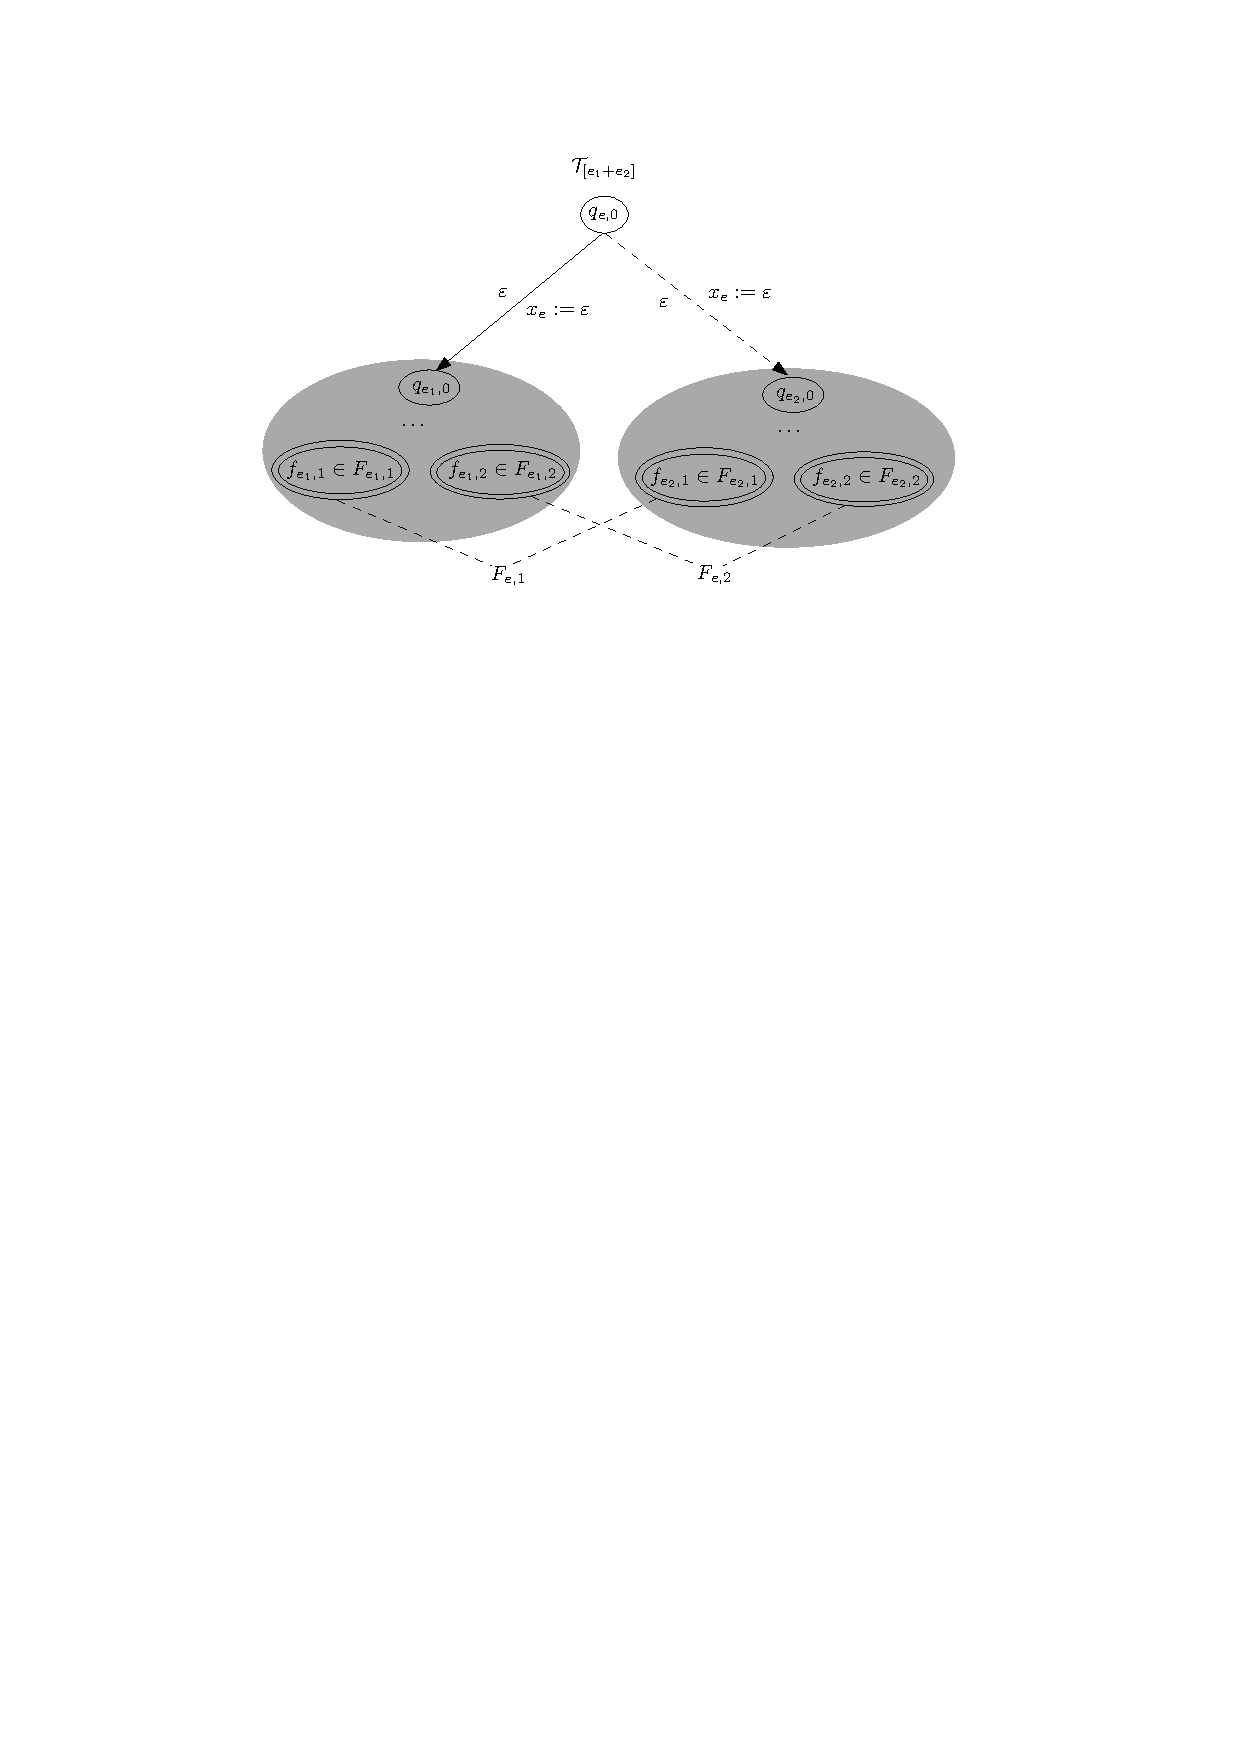
\includegraphics[width = 0.6\textwidth]{reg2pfa-1.pdf}
			\caption{The PSST $\cT_{[e_1+e_2]}$}
			\label{fig-reg2pfa-1}
			\vspace{-4mm}
		\end{figure}  


%%%%%%%%%%%%%%%%%%%%%%%%%%%%%%%%move to appendix %%%%%%%%%%%%%%%%%%%%%%%%%%%%%%%%%%%%%%%%%%%%%%%%%%%%%%%%%%%%%%%%%%%%%
%\paragraph{Case $e = [e_1 \concat e_2]$} 
%For $i \in \{1,2\}$, let  
%$\cT_{e_i} = (Q_{e_i}, \Sigma, X_{e_i}, \delta_{e_i}, \tau_{e_i}, E_{e_i}, q_{e_i,0}, (F_{e_i,1}, F_{e_i,2}))$. Moreover, let us assume that $X_{e_1}\cap X_{e_2}=\emptyset$.
%Then $\cT_e$ is obtained from $\cT_{e_1} \concat \cT_{e_2}$ (the concatenation of $\cT_{e_1}$ and $\cT_{e_2}$, see Figure~\ref{fig-psstconcat}) by adding a string variable $x_e$, a fresh state $q_{e,0}$ as the initial state, the transition $\tau_e(q_{e,0}) = (q_{e_1,0})$, and the assignments $E_e(q_{e,0}, \varepsilon, q_{e_1,0})(x_e) = \varepsilon$, $E_e(p, a, q)(x_e) = x_e a$ for every transition $(p, a, q)$ in $\cT_{e_1}$, $\cT_{e_2}$, and $\cT'_{e_2}$ (where $a \in \Sigma^\varepsilon$).
%%%%%%%%%%%%%%%%%%%%%%%%%%%%%%%
%\OMIT{
%Suppose that
%$\cT'_{e_2} = (Q'_{e_2}, \Sigma, X_{e_2}, \delta'_{e_2}, \tau'_{e_2}, E_{e_2}', q'_{e_2,0}, (F'_{e_2, 1}, F'_{e_2,2}))$ is a fresh copy of $\cT_{e_2}$, but with the string variables of $\cT_{e_2}$ kept unchanged. 
%Then 
%%
%\[\cT_e = ( Q_{e_1} \cup Q_{e_2} \cup Q'_{e_2} \cup \{q_{e,0}\}, \Sigma, X_e, \delta_e, \tau_e, q_{e_1,0}, (F_{e_2,1}, F_{e_2,2} \cup F'_{e_2,1} \cup F'_{e_2,2}))\] where 
%	\begin{itemize}
%	\item $X_e = X_{e_1} \cup X_{e_2} \cup \{x_e\}$,
%	%
%	\item $\delta_e$ is defined as follows:
%	\begin{itemize}
%	\item for every $a \in \Sigma$, $\delta_e(q_{e,0}, a) = ()$,
%	%
%	 \item for every $i \in \{1,2\}$, $q \in Q_{e_i}$ and $a \in \Sigma$, $\delta_e(q, a) = \delta_{e_i}(q, a)$,
%%
%	\item for every $q' \in Q'_{e_2}$ and $a \in \Sigma$, $\delta_e(q', a) = \delta'_{e_2}(q',a)$, 
%	 \end{itemize}
%			%
%	\item $\tau_e$ is defined as follows: 
%	\begin{itemize}
%	\item $\tau_e(q_{e,0}) = ((q_{e_1,0}); ())$;
%			%    
%	\item for every $q \in Q_{e_2}$, $\tau_e(q) = \tau_{e_2}(q)$ and $\tau_e(q') = \tau'_{e_2}(q')$, 
%			%
%	\item for every $q \in Q_{e_1} \setminus (F_{e_1,1} \cup F_{e_1,2})$, $\tau_e(q) = \tau_{e_1}(q)$, 
%	\item for every $f_{e_1,1} \in F_{e_1,1}$, $\tau_e(f_{e_1,1}) = ((q_{e_2,0}); ())$, 
%	\item for every $f_{e_1,2} \in F_{e_1,2}$, $\tau_e(f_{e_1,2}) = ((q'_{e_2,0}), ())$,
%	\end{itemize}
%	%
%	\item $E_e$ is defined as follows: 
%	\begin{itemize}
%	\item $E_e(q_{e,0}, \varepsilon, q_{e_1,0})(x_e) = \varepsilon$, and for every $x \in X_{e_1} \cup X_{e_2}$, $E_e(q_{e,0}, \varepsilon, q_{e_1,0})(x) = x$,
%	%
%	\item for each $i\in \{1,2\}$, transition $(p, a, q)$ in $\cT_{e_i}$ (where $a \in \Sigma^\varepsilon$), $E_e(p, a, q)(x_e) = x_e a$, moreover, for every $x\in X_{e_i}$, $E_e(p, a, q)(x) = E_{e_i}(p, a, q)(x)$,
%	%
%	\item for each transition $(p', a, q')$ in $\cT'_{e_2}$, $E_e(p', a, q')(x_e) = x_e a$, and for every $x \in X_{e_2}$, $E_e(p', a, q')(x) = E_{e_2}(p, a, q)(x)$,
%	\item for $f_{e_1,1} \in F_{e_1,1}$ and $f_{e_1,2} \in F_{e_1,2}$, $E_e(f_{e_1,1},\varepsilon,q_{e_2,0})(x_{e_2}) = E_e(f_{e_1,2},\varepsilon,q'_{e_2,0})(x_{e_2}) =\varepsilon$, and for every $x \in X_e \setminus \{x_{e_2}\}$, $E_e(f_{e_1,1},\varepsilon,q_{e_2,0})(x) = E_e(f_{e_1,2},\varepsilon,q'_{e_2,0})(x) = x$.
%	\end{itemize}
%  \end{itemize}
% }
% %%%%%%%%%%%%%%%%%%%%%%%%%%%%%%
%% Fig.~\ref{fig-reg2pfa-2} depicts the construction. 
%\begin{figure}[ht]
%			\centering
%			%\rule{\linewidth}{0cm}
%			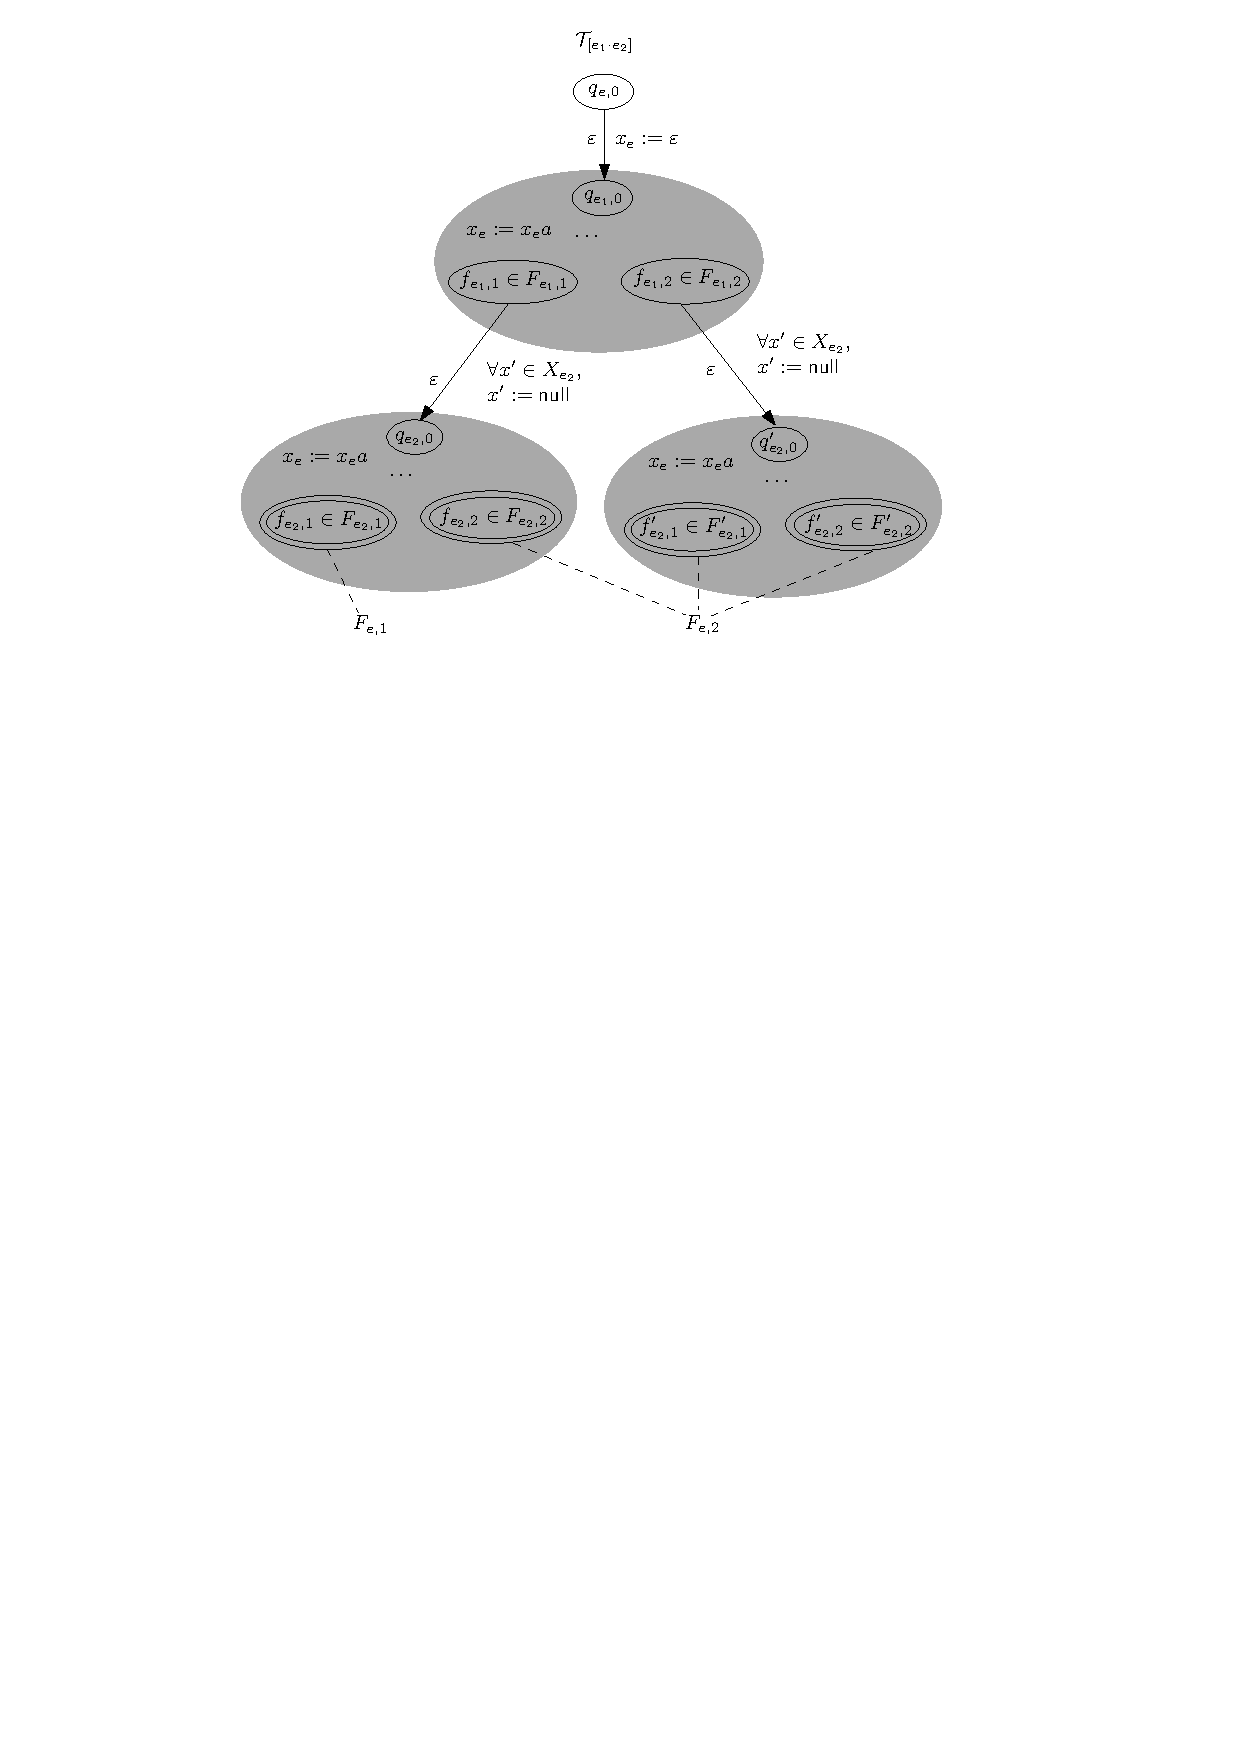
\includegraphics[width = 0.6\textwidth]{reg2pfa-2.pdf}
%			\caption{The PSST $\cT_{[e_1\concat e_2]}$}
%			\label{fig-reg2pfa-2}
%\end{figure}  
%	
%%%%%%%%%%%%%%%%%%%%%%%%%%%% move to appendix %%%%%%%%%%%%%%%%%%%%%%%%%%%%%%%%%%%%%%%%%%%%%%%%%%%%%%%%%%%%%%%%%%%%%%%%%

\paragraph{Case $e = [e_1 \concat e_2]$} 
For $i \in \{1,2\}$, let  
$\cT_{e_i} = (Q_{e_i}, \Sigma, X_{e_i}, \delta_{e_i}, \tau_{e_i}, E_{e_i}, q_{e_i,0}, (F_{e_i,1}, F_{e_i,2}))$. Moreover, let us assume that $X_{e_1}\cap X_{e_2}=\emptyset$.
Then $\cT_e$ is obtained from $\cT_{e_1} \concat \cT_{e_2}$ (the concatenation of $\cT_{e_1}$ and $\cT_{e_2}$, see Figure~\ref{fig-psstconcat}) by adding a string variable $x_e$, a fresh state $q_{e,0}$ as the initial state, the $\varepsilon$-transition $\tau_e(q_{e,0}) = ((q_{e_1,0});())$, and the assignments $E_e(q_{e,0}, \varepsilon, q_{e_1,0})(x_e) = \varepsilon$, $E_e(p, a, q)(x_e) = x_e a$ for every transition $(p, a, q)$ in $\cT_{e_1}$, $\cT_{e_2}$, and $\cT'_{e_2}$ (where $a \in \Sigma^\varepsilon$).


\paragraph{Case $e = [e_1^?]$ (see Figure~\ref{fig-reg2pfa-6})} Let $\cT_{e_1} = (Q_{e_1}, \Sigma, X_{e_1}, \delta_{e_1}, \tau_{e_1}, E_{e_1}, q_{e_1,0}, (F_{e_1,1}, F_{e_1,2}))$. Then 
\[\cT_e = (Q_{e_1} \cup \{q_{e,0}, f_{\varepsilon}\}, \Sigma, X_{e_1} \cup \{x_e\}, 
		\delta_e, \tau_e, E_{e}, q_{e,0}, (\{f_{\varepsilon}\}, F_{e_1,2}))\]
where  
		\begin{itemize}
%			\item $q_{e,0}, f_\varepsilon  \not \in Q_{e_1}$,
			\item $\delta_e$ is exactly $\delta_{e_1}$,
%			\begin{itemize}
%			\item $\delta_e(q, a) = \delta_{e_1}(q, a)$ for every $q \in Q_{e_1}$ and $a \in \Sigma$, 
%			\item $\delta_e(q_{e,0}, a)  = ()$ and $\delta_e(f_{\varepsilon}, a) = ()$ for every $a \in \Sigma$, 
%			\end{itemize}
			%
			\item $\tau_e$ comprises the transitions in $\tau_{e_1}$, as well as the transition $\tau_e(q_{e,0}) = ((q_{e_1,0}, f_{\varepsilon}); ())$,
%			\begin{itemize}
%			\item $\tau_e(q) = \tau_{e_1}(q)$ for every $q \in Q_{e_1}$, 
%			\item $\tau_e(q_{e,0}) = ((q_{e_1,0}, f_{\varepsilon}); ())$,
%			\end{itemize}
			\item $E_e$ inherits $E_{e_1}$ and the assignments $E_e(q_{e,0},\varepsilon,q_{e_1, 0})(x_e) = E_e(q_{e,0},\varepsilon,f_{\varepsilon})(x_e) =\varepsilon$, as well as $E_e(q, a, q')(x_e) =x_e a$ for every transition $(q, a, q')$ in $\cT_{e_1}$ (where $a \in \Sigma^\varepsilon$).
%			defined as follows: 
%			\begin{itemize}
%			\item for each transition $(q, a, q')$ in $\cT_{e_1}$ (where $a \in \Sigma^\varepsilon$), $E_e(q,a,q')(x_e) =x_ea$, and for every $x \in X_{e_1}$, $E_e(q,a,q')(x) =E_{e_1}(q, a,q')(x)$, 
			%
%			\item $E_e(q_{e,0},\varepsilon,q_{e_1, 0})(x_e) = E_e(q_{e,0},\varepsilon,f_{\varepsilon})(x_e) =\varepsilon$,  and for each $x \in X_{e_1}$, $E_e(q_{e,0},\varepsilon,q_{e_1, 0})(x)  = E_e(q_{e,0},\varepsilon, f_{\varepsilon})(x) =x$. 
%			\end{itemize}
		\end{itemize}
%
%Fig.~\ref{fig-reg2pfa-6} depicts the construction.
		\begin{figure}[tb]
		\vspace{-2mm}
			\centering
			%\rule{\linewidth}{0cm}
			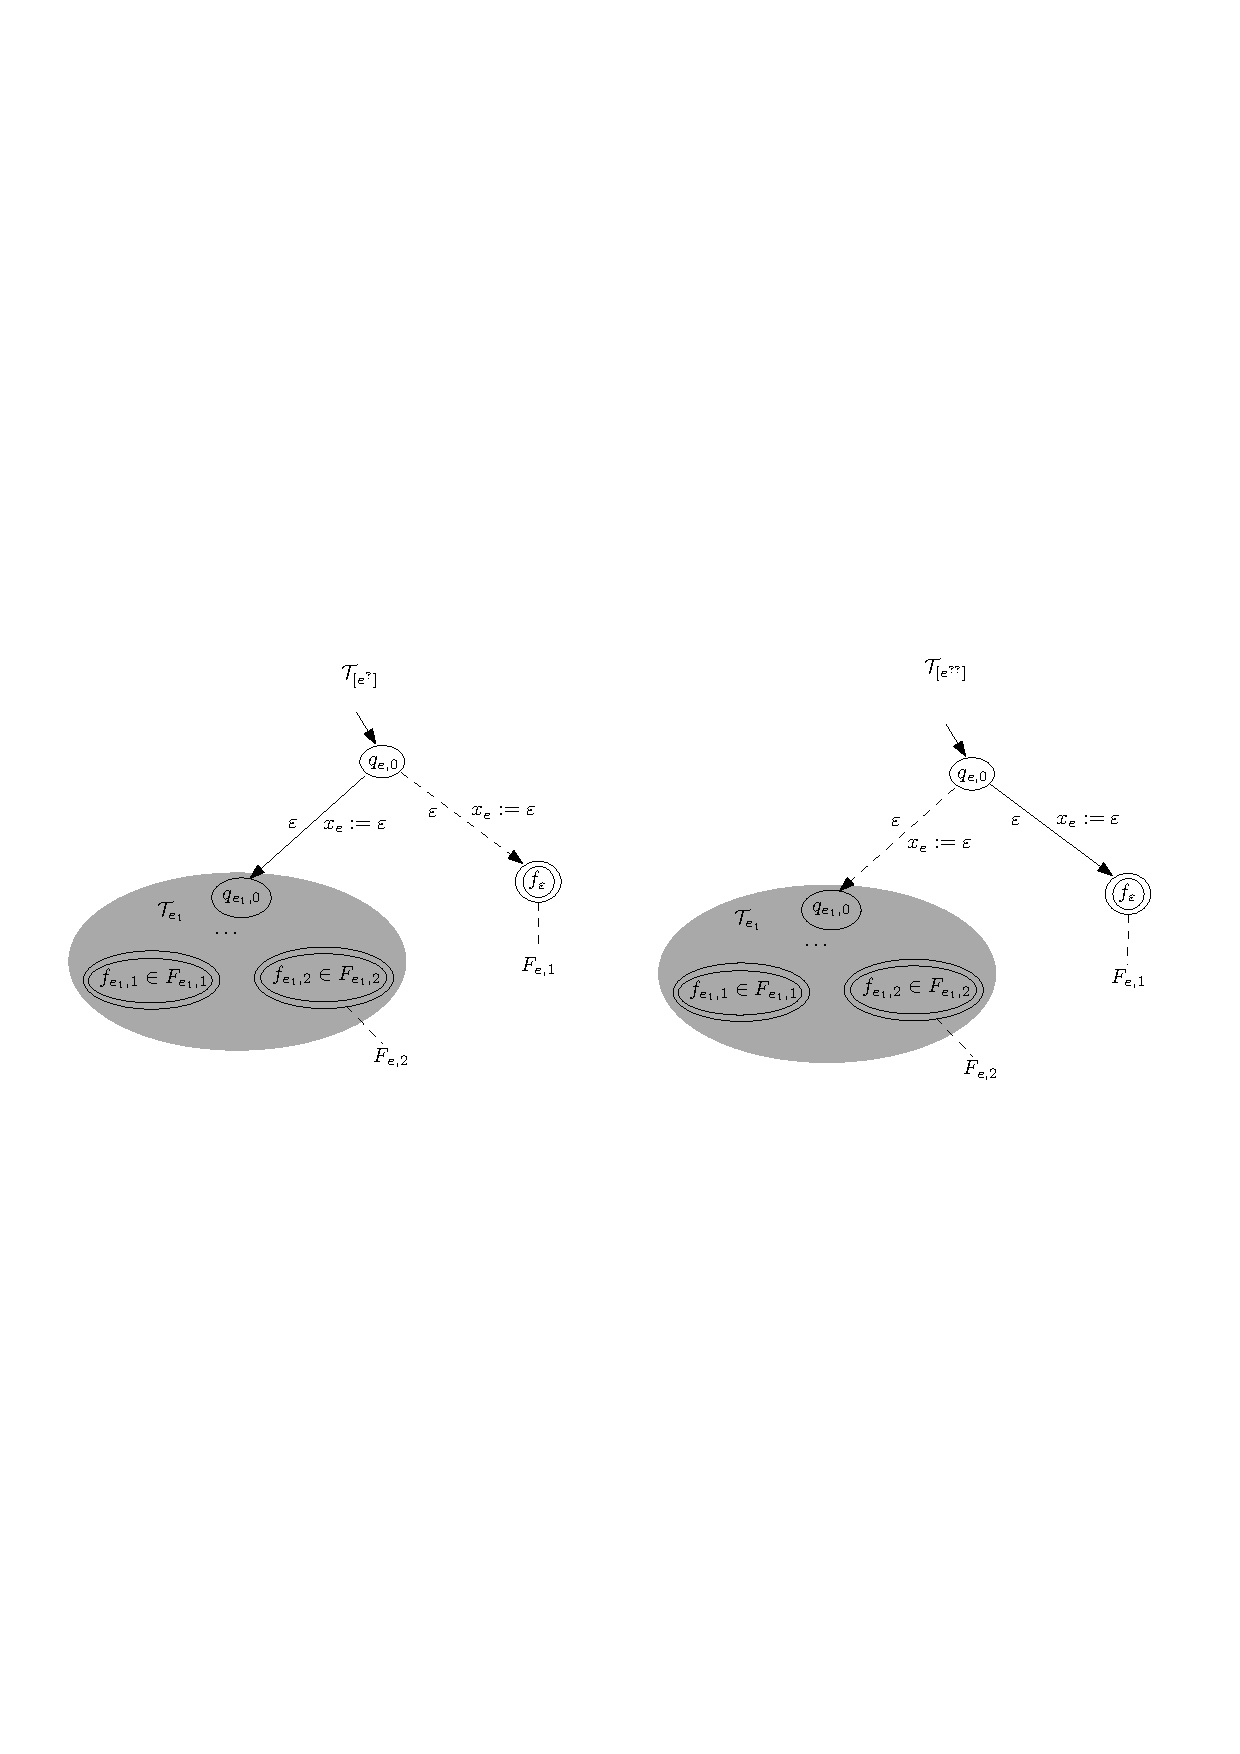
\includegraphics[width = 0.8\textwidth]{reg2pfa-6.pdf}
			\caption{The PSST $\cT_{[e_1^?]}$ and $\cT_{[e_1^{??}]}$}
			\label{fig-reg2pfa-6}
			\vspace{-4mm}
		\end{figure}

%%%%%%%%%%%%%%%%%%%%%%%%%%%%%%%%%%%%%%%%%%%%%%%%%%%%%%%%%%%%%%%%%%%%%%%%%%%%%%%%%%%%%%%%%%%%%%%%%%%%%
\paragraph{Case $e = [e_1^{??}]$ (see Figure~\ref{fig-reg2pfa-6})}  In this case, $\cT_{[e_1^{??}]}$ is  almost the same as $\cT_{[e_1^{?}]}$. The only difference is that the priorities of the two $\varepsilon$-transitions out of $q_{e,0}$ are swapped, namely, $\tau_e(q_{e,0}) = ((f_{\varepsilon}, q_{e_1,0}); ())$ here.
%%%%%%%%%%%%%%%%%%%%%%%%%%%%%%%%%%%%%%%
\OMIT
{
Let $\cT_{e_1} = (Q_{e_1},
		\Sigma, X_{e_1}, \delta_{e_1}, \tau_{e_1}, E_{e_1} , q_{e_1,0}, (F_{e_1,1}, F_{e_1,2}))$. 
Then 
\[\cA_e = (Q_{e_1} \cup \{q_{e,0}, q_{\varepsilon}\}, \Sigma, X, 
		\delta_e, \tau_e, E, q_{e,0}, (\{q_{\varepsilon}\}, F_{e_1,2}))\] 
where 
		\begin{itemize}
			\item $q_{e,0}  \not \in Q_{e_1}$
			\item $\delta_e(q, a) = \delta_{e_1}(q, a)$ for every $q \in Q_{e_1}$ and $a \in \Sigma$, $\delta_e(q_{e,0}, a)  = ()$ and $\delta_e(q_{\varepsilon}, a) = ()$ for every $a \in \Sigma$, 
			%
			\item $\tau_e(q) = \tau_{e_1}(q)$ for every $q \in Q_{e_1}$, $\tau_e(q_{e,0}) = ((q_{\varepsilon}, q_{e_1,0}); ())$,
			
			\item for each transition $(q, a, q')$ from $\delta_{e_1}$, $E(q,a,q')(x) = E_1(q,a,q')(x)$ and $E(q_{e,0},\varepsilon,q_{\varepsilon})(x) =\varepsilon$
		\end{itemize}
}
%%%%%%%%%%%%%%%%%%%%%%%%%%%%%%%%%%%%%%%
\OMIT{
Fig.~\ref{fig-reg2pfa-7} depicts the construction. 
		\begin{figure}[ht]
			\centering
			%\rule{\linewidth}{0cm}
			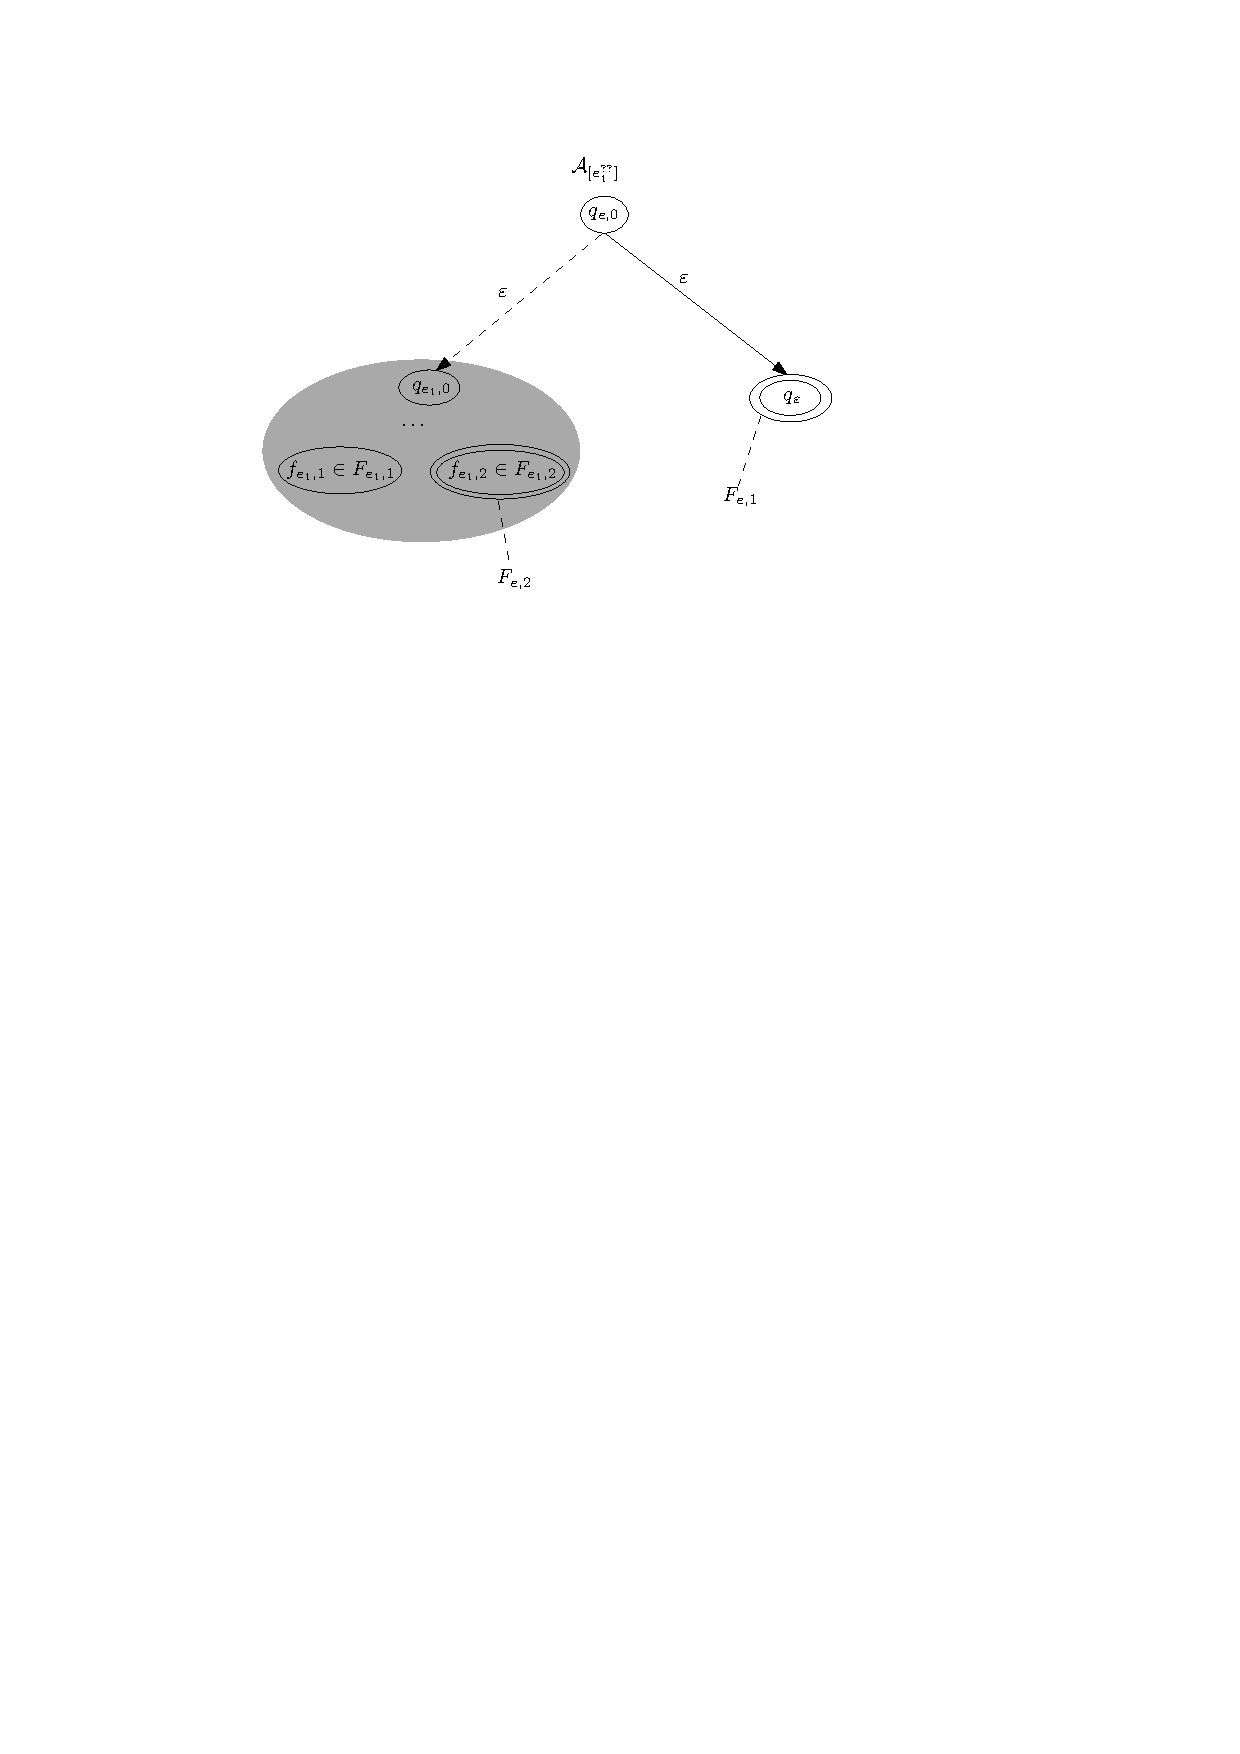
\includegraphics[width = 0.5\textwidth]{reg2pfa-7.pdf}
			\caption{The PFA $\cA_{[e_1^{??}]}$}
			\label{fig-reg2pfa-7}
		\end{figure}
}	

%%%%%%%%%%%%%%%%%%%%%%%%%%%%%%%%%%%%%%%%%%%%%%%%%%%%%%%%%%%%%%%%%%%%%%%%%%%%%%%%%%%%%%%%%%%%%%%%%%%%%

\paragraph{Case $e = [e_1^{\ast}]$ (see Figure~\ref{fig-reg2pfa-3})} 
Let $\cT_{e_1} = (Q_{e_1}, \Sigma, X_{e_1}, \delta_{e_1}, \tau_{e_1}, E_{e_1}, q_{e_1,0}, (F_{e_1,1}, F_{e_1,2}))$. Then
\[ \cT_e = (Q_{e_1} \cup \{q_{e,0}, f_{e,1}, f_{e,2}\}, \Sigma, X_{e}, \delta_e, E_{e}, \tau_e, q_{e,0}, (\{f_{e,1}\}, \{f_{e,2}\}))\] where 
		\begin{itemize}
%			\item $q_{e,0}, f_{e,1}, f_{e,2} \not \in Q_{e_1}$,
			
			\item $\delta_e$ is exactly $\delta_{e_1}$,
%			 defined as follows:
%			\begin{itemize}
%			\item for every $q \in Q_{e_1}$ and $a \in \Sigma$, $\delta_e(q, a) = \delta_{e_1}(q, a)$, 
%			\item for every $a \in \Sigma$, $\delta_e(q_{e,0}, a) = \delta_e(f_{e,0}, a) = \delta_e(f_{e,1}, a) = ()$,
%			\end{itemize}
			%moreover, $\delta(q_0, a) = \delta(f_0, a)  = ()$,
%
			\item $\tau_e$ comprises the transitions in $\tau_{e_1}$,  as well as the transitions $\tau_e(q_{e,0}) = ((q_{e_1,0}, f_{e,1}); ())$,  $\tau_e(f_{e_1,1}) = ((q_{e_1,0});())$ for every $f_{e_1,1} \in F_{e_1,1}$, and $\tau_e(f_{e_1,2}) = ((q_{e_1,0}, f_{e,2});())$ for every $f_{e_1,2} \in F_{e_1,2}$, 
%			defined as follows: 
%			\begin{itemize}
%			\item for every $q \in Q_{e_1} \setminus (F_{e_1,1} \cup F_{e_1,2})$,  $\tau_e(q) = \tau_{e_1}(q)$, moreover, $\tau_e(q_{e,0}) = ((q_{e_1,0},f_{e,0}); ())$,  $\tau_e(f_{e_1,1}) = ((q_{e_1,0});())$ for every $f_{e_1,1} \in F_{e_1,1}$, $\tau_e(f_{e_1,2}) = ((q_{e_1,0}, f_{e,1});())$ for every $f_{e_1,2} \in F_{e_1,2}$, $\tau_e(f_{e,0}) =\tau_e(f_{e,1}) = (();())$. (Intuitively, the $\varepsilon$-transitions from $q_{e,0}$ to $q_{e_1,0}$ and $f_{e,0}$, from each $f_{e_1,1} \in F_{e_1,1}$ to $q_{e_1,0}$, and from $f_{e_1,2} \in F_{e_1,2}$ to $q_{e_1,0}$ and $f_{e,1}$ respectively are added, moreover, the $\varepsilon$-transition from $q_{e,0}$ to $f_{e,0}$ and from $f_{e_1,2} \in F_{e_1,2}$ to $f_{e,1}$ are of the lowest priority.)
%			\end{itemize}
			\item $E_e$ inherits $E_{e_1}$ and the assignments $E_e(q_{e,0},\varepsilon,f_{e,1})(x_e) = E_e(q_{e,0},\varepsilon,q_{e_1,0})(x_e) = \varepsilon$, as well as $E_e(f_{e_1,1},\varepsilon, q_{e_1,0})(x) = E_e(f_{e_1,2},\varepsilon, q_{e_1,0})(x)= \nullchar$ for every $f_{e_1,1} \in F_{e_1,1}$, $f_{e_1,2} \in F_{e_1,2}$, and $x \in X_{e_1}$. (Intuitively, the values of all the string variables in $X_{e_1}$ are reset when starting a new iteration of $e_1$.)
%			 is defined as follows: 
%			\begin{itemize}
%			\item for each transition $(q, a, q')$ in $\cT_{e_1}$, $E_e(q,a,q')(x_e) = x_e a$, and for every $x \in X_{e_1}$, $E_e(q,a,q')(x) = E_{e_1}(q,a,q')(x)$, 
%			\item $E_e(q_{e,0},\varepsilon,f_{e,0})(x_e) = E_e(q_{e,0},\varepsilon,q_{e_1,0})(x_e) = \varepsilon$, and for every $x \in X_{e_1}$, $E_e(q_{e,0},\varepsilon,f_{e,0})(x) = E_e(q_{e,0},\varepsilon,q_{e_1,0})(x) = x$, 
%			\item for every $f_{e_1,1} \in F_{e_1,1}$, $E_e(f_{e_1,1},\varepsilon,q_{e_1,0})(x_{e}) = \varepsilon$, and for every $x \in X_{e_1}$, $E_e(f_{e_1,1},\varepsilon,q_{e_1,0})(x) =x$, 
%			\item for every $f_{e_1,2} \in F_{e_1,2}$, $E_e(f_{e_1,1},\varepsilon,q_{e_1,0})(x_{e}) = \varepsilon$, $E_e(f_{e_1,2},\varepsilon,f_{e,1})(x_{e}) = x_e$, and for every $x \in X_{e_1}$, $E_e(f_{e_1,2},\varepsilon,q_{e_1,0})(x) = E(f_{e_1,2},\varepsilon, f_{e,1})(x) = x$.
%			\end{itemize}
		\end{itemize}

%Fig.~\ref{fig-reg2pfa-3} depicts the construction. 
\begin{figure}[tb]
	\centering
	%\rule{\linewidth}{0cm}
	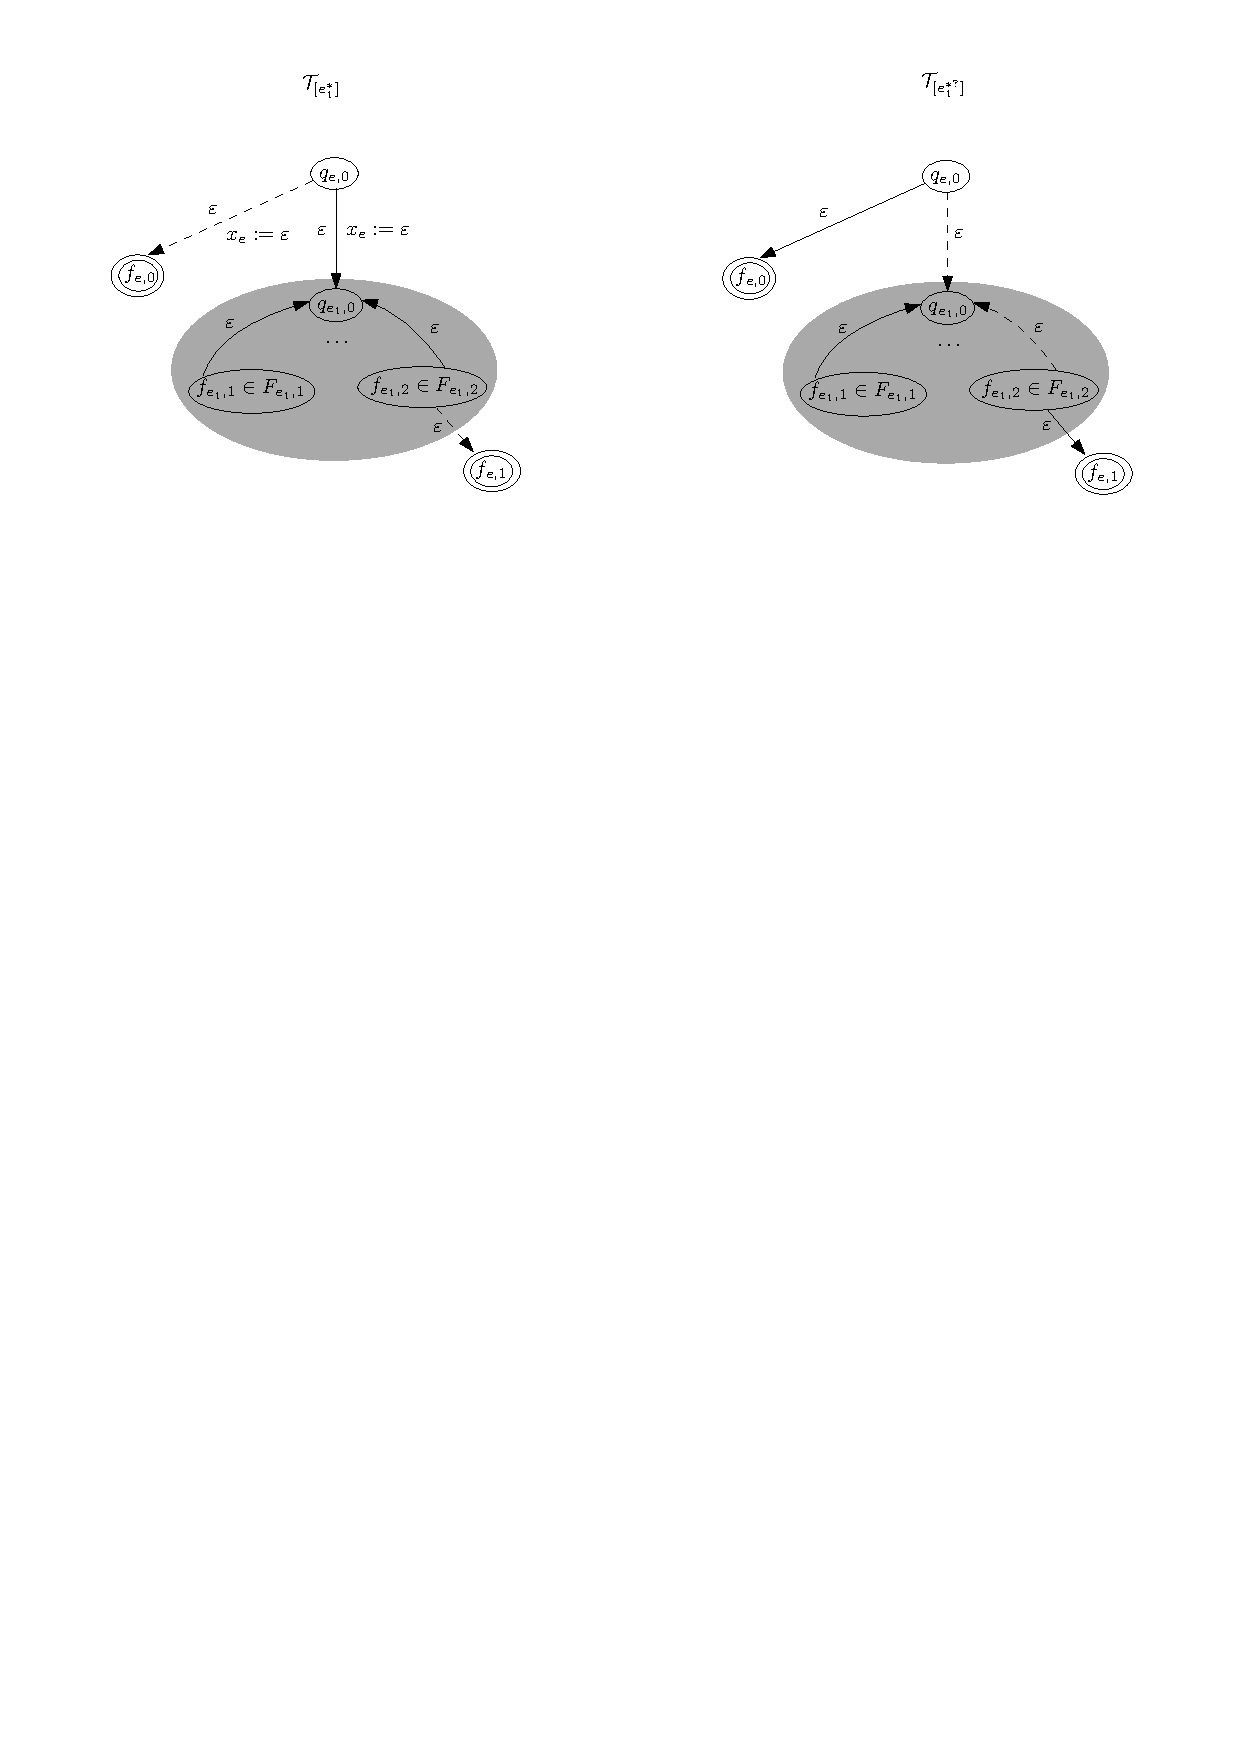
\includegraphics[width = 0.8\textwidth]{reg2pfa-3.pdf}
	\caption{The PSST $\cT_{[e_1^\ast]}$ and $\cT_{[e_1^{\ast?}]}$}
	\label{fig-reg2pfa-3}
	\vspace{-4mm}
\end{figure}

%%%%%%%%%%%%%%%%%%%%%%%%%%%%%%%%%%%%%%%%%%%%%%%%%%%%%%%%%%%%%%%%%%%%%%%%%%%%%%%%%%%%%%%%%%%%%%%%%%%%%
\paragraph{Case $e = [e_1^{\ast?}]$ (see Figure~\ref{fig-reg2pfa-3})} The construction is almost the same as $e = [e_1^{\ast}]$. The only difference is that the priorities of the $\varepsilon$-transitions out of $q_{e,0}$ resp. $f_{e_1,2} \in F_{e_1,2}$ are swapped.
%
\OMIT{
Let $\cA_{e_1} = (Q_{e_1}, \Sigma, X_1, \delta_{e_1}, \tau_{e_1}, E_1, q_{e_1,0}, (F_{e_1,1}, F_{e_1,2}))$. 
Then 
\[\cA_e = (Q_{e_1} \cup \{q_{e,0}, f_{e,0}, f_{e,1}\}, \Sigma, X_1, \delta_e, \tau_e, E, q_{e,0}, (\{f_{e,0}\}, \{f_{e,1}\}))\]  
where 
		\begin{itemize}
			\item $q_{e,0}, f_{e,0} \not \in Q_{e_1}$,
			
			\item for every $q \in Q_{e_1}$ and $a \in \Sigma$, $\delta_e(q, a) = \delta_{e_1}(q, a)$, 
			%moreover, $\delta(q_0, a) = \delta(f_0, a)  = ()$,
			
			\item for every $q \in Q_{e_1} \setminus (F_{e_1,1} \cup F_{e_1,2})$,  $\tau_e(q) = \tau_{e_1}(q)$, moreover, $\tau_e(q_{e,0}) = ((f_{e,0}, q_{e_1,0}); ())$,  $\tau_e(q) = ((q_{e_1,0});())$ for every $q \in F_{e_1,1}$, $\tau_e(q) = ((f_{e,1}, q_{e_1,0});())$ for every $q \in F_{e_1,2}$, $\tau_e(f_{e,0}) =\tau_e(f_{e,1}) = (();())$. (Intuitively, the $\varepsilon$-transitions from $q_{e,0}$ to $f_{e,0}$ and $q_{e_1,0}$ , from each $q \in F_{e_1,1}$ to  $q_{e_1,0}$, and from each $q \in F_{e_1,2}$ to $f_{e,1}$ and $q_{e_1,0}$ respectively are added, moreover, the $\varepsilon$-transition from $q_{e,0}$ to $q_{e_1,0}$ and from $q \in F_{e_1,2}$ to $q_{e_1,0}$ are of the lowest priority.)
			
			\item for each transition $(q, a, q')$ from $\delta_{e_1}$, $E(q,a,q')(x) = E_1(q,a,q')(x)$, and $E(q_{e,0},\varepsilon,q_{f_e,0})(x) =\varepsilon$, $E(q_{e,0},\varepsilon,q_{e_1,0})(x) =\varepsilon$, $E(f_{e_1,2},\varepsilon,f_{e,1})(x) =x$.
		\end{itemize}
}


\paragraph{Case $e = [e_1^{+}]$}  We first construct $\cT_{e_1}$ and $\cT^-_{[e^\ast_1]}$, where $\cT^-_{[e^\ast_1]}$ is obtained from $\cT_{[e^\ast_1]}$ by dropping the string variable $x_{[e^\ast_1]}$. Therefore, $\cT_{e_1}$ and $\cT^-_{[e^\ast_1]}$ have the same set of string variables, $X_{e_1}$. Then we construct $\cT_{e}$ by adding into $\cT_{e_1} \concat \cT^-_{[e^\ast_1]}$ a fresh state $q_{e,0}$ as the initial state, and the transitions $\tau_e(q_{e,0}) = ((q_{e_1,0});())$, as well as the assignments $E_e(q_{e,0}, \varepsilon, q_{e_1,0})(x_e) = \varepsilon$, $E_e(p, a, q)(x_e) = x_e a$ for every transition $(p, a, q)$ in $\cT_{e_1} \concat \cT^-_{[e^\ast_1]}$. 
%(Note that in $\cT_{e_1} \concat \cT^-_{[e^\ast_1]}$, the values of all variables in $X_{e_1}$ are reset when entering $ \cT^-_{[e^\ast_1]}$ and $(\cT^-_{[e^\ast_1]})'$.)

%%%%%%%%%%%%%%%%%%%%%%%%%%%%%%%%%%%%%%%%%%%%%%%%%%%%%%%%%%%%%%%%%%%%%%%%%%%%%%%%%%%%%%%%%%%%%%%%%%%%%
\paragraph{Case $e = [e_1^{\{m_1,m_2\}}]$ for $1 \le m_1 < m_2$ (see Figure~\ref{fig-reg2pfa-4})} We first construct $\cT^{\{m_1\}}_{e_1}$ as the concatenation of $m_1$ copies of $\cT_{e_1}$ (Recall Definition~\ref{def-psstconcat} for the concatenation of PSSTs). Note that $\cT^{\{m_1\}}_{e_1}$ is different from $\cT_{e_1^{m_1}}$, the PSST constructed from $e_1^{m_1}$, the concatenation of the expression $e_1$ for $m_1$ times. In particular, the set of string variables in $\cT^{\{m_1\}}_{e_1}$ is $X_{e_1}$, which is different from that of $\cT_{e_1^{m_1}}$. 

Then we construct the PSST $\cT^{\{1,m_2-m_1\}}_{e_1}$ (see Fig.~\ref{fig-reg2pfa-4}), which consists of $m_2-m_1$ copies of $\cT_{e_1}$, denoted by $(\cT^{(i)}_{e_1})_{i \in [m_2-m_1]}$, as well as the $\varepsilon$-transition from $q^{(1)}_{e_1,0}$ to a fresh state $f^\prime_0$ (of the lowest priority), and the $\varepsilon$-transitions from each $f^{(i)}_{e_1,2} \in F^{(i)}_{e_1,2}$ with $1\le i < m_2-m_1$ to $q^{(i+1)}_{e_1,0}$ (of the highest priority) and a fresh state $f^\prime_1$ (of the lowest priority). The final states of $\cT^{\{1,m_2-m_1\}}_{e_1}$ are $(\{f_0'\},\{f_1'\})$. (Intuitively, each $\cT^{(i)}_{e_1}$ accepts only nonempty strings, thus $f^{(i)}_{e_1,1} \in F^{(i)}_{e_1,1}$ contains no outgoing transitions in $\cT^{\{1,m_2-m_1\}}_{e_1}$. ) Note that the set of string variables in $\cT^{\{1,m_2-m_1\}}_{e_1}$ is still $X_{e_1}$.
%
\begin{figure}[tb]
	\vspace{-2mm}
	\centering
	%\rule{\linewidth}{0cm}
	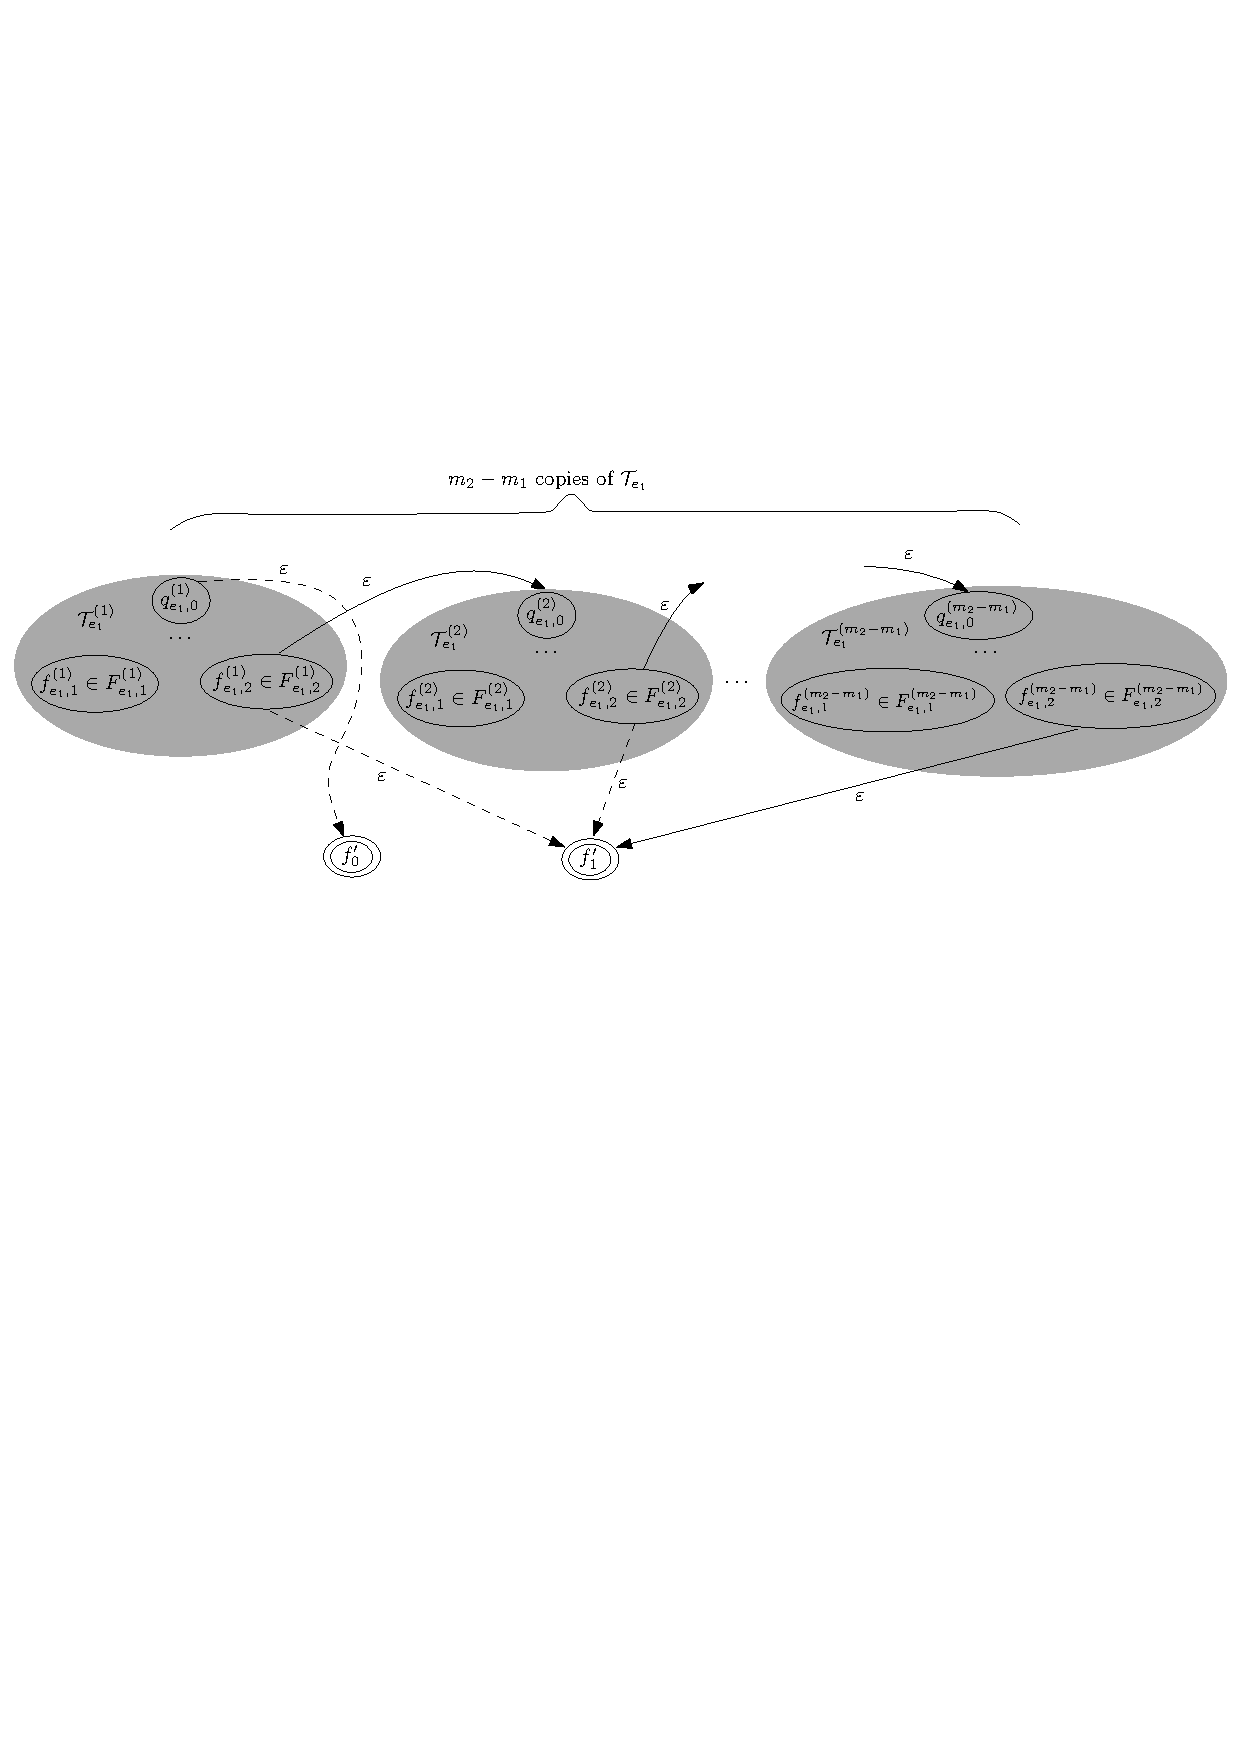
\includegraphics[width = 0.8\textwidth]{reg2pfa-4.pdf}
	\caption{The PSST $\cT^{\{1,m_2-m_1\}}_{e_1}$}
	\label{fig-reg2pfa-4}
	\vspace{-4mm}
\end{figure}  

Finally, we construct $\cT_e$ from $\cT^{\{m_1\}}_{e_1} \concat \cT^{\{1,m_2-m_1\}}_{e_1}$, the concatenation of $\cT^{\{m_1\}}_{e_1}$ and $\cT^{\{1,m_2-m_1\}}_{e_1}$, by adding a fresh state $q_{e,0}$, a string variable $x_e$, the $\varepsilon$-transition $\tau_e(q_{e,0}) = ((q_{e_1,0});())$ (assuming that $q_{e_1,0}$ is the initial state of $\cT^{\{m_1\}}_{e_1}$),  and the assignments $E_e(q_{e_0}, \varepsilon, q_{e_1,0})(x_e) = \varepsilon$, as well as $E_e(p, a, q)(x_e) = x_e a$ for each transition $(p, a, q)$ in  $\cT^{\{m_1\}}_{e_1} \concat \cT^{\{1,m_2-m_1\}}_{e_1}$.

%%%%%%%%%%%%%%%%%%%%%%%%%%%%%%%%%%%% move to appendix %%%%%%%%%%%%%%%%%%%%%%%%%%%%%%%%%%%%%%%%%%%%%%%%%%%%%%%%%%%%%%%%%
%\paragraph{Case $e = [e_1^{+}]$}  We first construct $\cT_{e_1}$ and $\cT^-_{[e^\ast_1]}$, where $\cT^-_{[e^\ast_1]}$ is obtained from $\cT_{[e^\ast_1]}$ by dropping the string variable $x_{[e^\ast_1]}$. Therefore, $\cT_{e_1}$ and $\cT^-_{[e^\ast_1]}$ have the same set of string variables, $X_{e_1}$. Then we construct $\cT_{e}$ by adding into $\cT_{e_1} \concat \cT^-_{[e^\ast_1]}$, the concatenation of $\cT_{e_1}$ and $\cT^-_{[e^\ast_1]}$, a fresh state $q_{e,0}$ as the initial state, and the transitions $\tau_e(q_{e,0}) = ((q_{e_1,0});())$, as well as the assignments $E_e(q_{e,0}, \varepsilon, q_{e_1,0})(x_e) = \varepsilon$, $E_e(p, a, q)(x_e) = x_e a$ for every transition $(p, a, q)$ in $\cT_{e_1} \concat \cT^-_{[e^\ast_1]}$. (Note that in $\cT_{e_1} \concat \cT^-_{[e^\ast_1]}$, the values of all variables in $X_{e_1}$ are reset when entering $ \cT^-_{[e^\ast_1]}$ and $(\cT^-_{[e^\ast_1]})'$.)
%
%% follows: We first construct $\cT_{[e_1 \concat [e^\ast_1]]}$. Since $[e_1 \concat [e^\ast_1]]$ is the concatenation of $e_1$ and $[e^\ast_1]$, each subexpression $e'$ of $e_1$ occurs twice in $[e_1 \concat [e^\ast_1]]$. Therefore for each subexpression $e'$ of $e_1$, $\cT_{[e_1 \concat [e^\ast_1]]}$ contains two string variables $x_{e'}$ and $x'_{e'}$, for the two occurrences of $e'$ in $e_1$  and $[e^\ast_1]$ respectively. Then we obtain $\cT_e$  from $\cT_{[e_1 \concat [e^\ast_1]]}$ by replacing $x'_{e'}$  with $x_{e'}$ for each subexpression $e'$ of $e_1$. 
%		
%
% 
%%%%%%%%%%%%%%%%%%%%%%%%%%%%%%%%%%%%%%%%%%%%%%%%%%%%%%%%%%%%%%%%%%%%%%%%%%%%%%%%%%%%%%%%%%%%%%%%%%%%%%
%\paragraph{Case $e = [e_1^{+?}]$} Then $\cT_e$ is constructed from $\cT_{e_1}$ and $\cT^-_{[e^{\ast?}_1]}$, similarly to the aforementioned construction of $\cT_{[e_1^{+}]}$.
%
%
%%%%%%%%%%%%%%%%%%%%%%%%%%%%%%%%%%%%%%%%%%%%%%%%%%%%%%%%%%%%%%%%%%%%%%%%%%%%%%%%%%%%%%%%%%%%%%%%%%%%%%
%\paragraph{Case $e = [e_1^{\{m_1,m_2\}}]$ for $1 \le m_1 < m_2$ (see Figure~\ref{fig-reg2pfa-4})} We first construct $\cT^{\{m_1\}}_{e_1}$ as the concatenation of $m_1$ copies of $\cT_{e_1}$ (Recall Definition~\ref{def-psstconcat} for the concatenation of PSSTs). Note that $\cT^{\{m_1\}}_{e_1}$ is different from $\cT_{e_1^{m_1}}$, the PSST constructed from $e_1^{m_1}$, the concatenation of the expression $e_1$ for $m_1$ times. In particular, the set of string variables in $\cT^{\{m_1\}}_{e_1}$ is $X_{e_1}$, which is different from that of $\cT_{e_1^{m_1}}$. 
%
%Then we construct the PSST $\cT^{\{1,m_2-m_1\}}_{e_1}$ (see Fig.~\ref{fig-reg2pfa-4}), which consists of $m_2-m_1$ copies of $\cT_{e_1}$, denoted by $(\cT^{(i)}_{e_1})_{i \in [m_2-m_1]}$, as well as the $\varepsilon$-transition from $q^{(1)}_{e_1,0}$ to a fresh state $f^\prime_0$ (of the lowest priority), and the $\varepsilon$-transitions from each $f^{(i)}_{e_1,2} \in F^{(i)}_{e_1,2}$ with $1\le i < m_2-m_1$ to $q^{(i+1)}_{e_1,0}$ (of the highest priority) and a fresh state $f^\prime_1$ (of the lowest priority). The final states of $\cT^{\{1,m_2-m_1\}}_{e_1}$ are $(\{f_0'\},\{f_1'\})$. (Intuitively, each $\cT^{(i)}_{e_1}$ accepts only nonempty strings, thus $f^{(i)}_{e_1,1} \in F^{(i)}_{e_1,1}$ contains no outgoing transitions in $\cT^{\{1,m_2-m_1\}}_{e_1}$. ) Note that the set of string variables in $\cT^{\{1,m_2-m_1\}}_{e_1}$ is still $X_{e_1}$.
%		%
%		\begin{figure}[ht]
%			\centering
%			%\rule{\linewidth}{0cm}
%			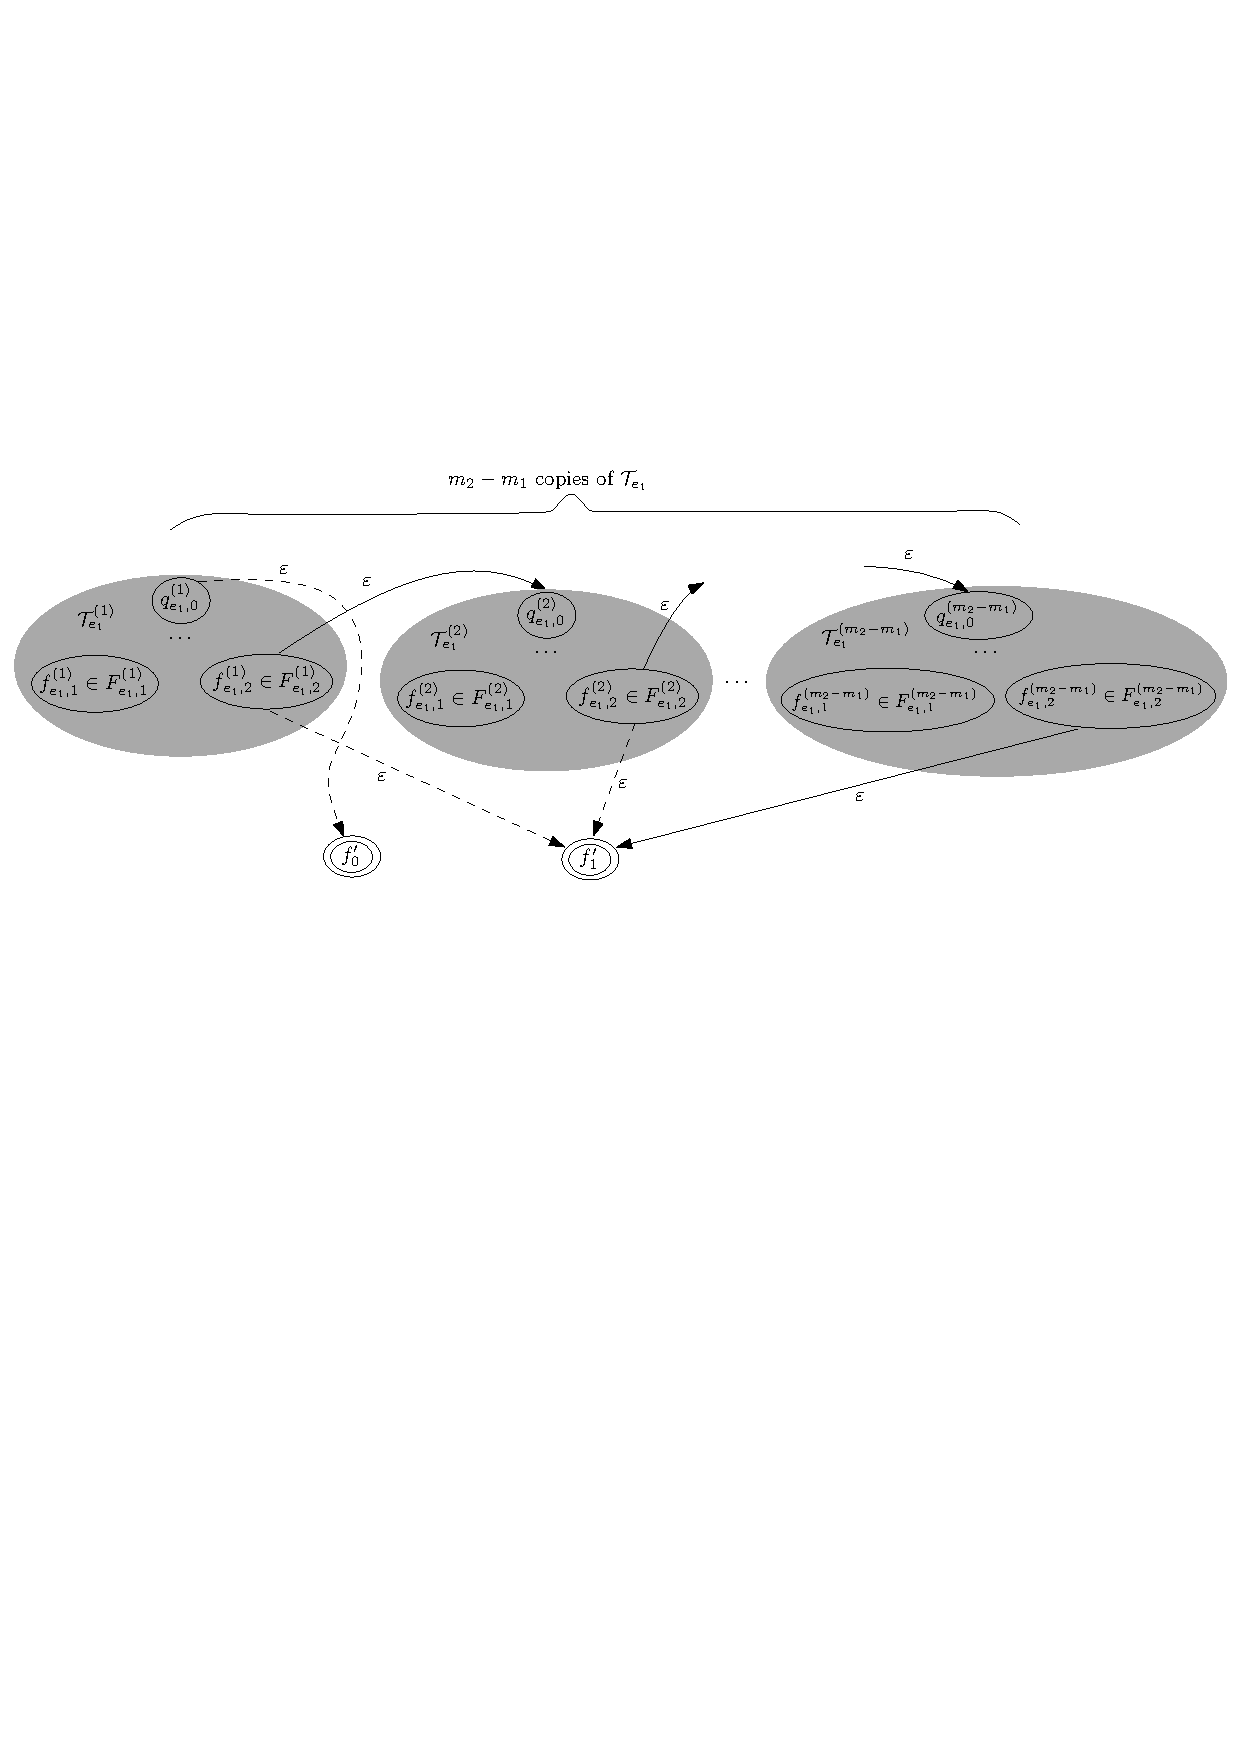
\includegraphics[width = 0.8\textwidth]{reg2pfa-4.pdf}
%			\caption{The PSST $\cT^{\{1,m_2-m_1\}}_{e_1}$}
%			\label{fig-reg2pfa-4}
%		\end{figure}  
%
%Finally, we construct $\cT_e$ from $\cT^{\{m_1\}}_{e_1} \concat \cT^{\{1,m_2-m_1\}}_{e_1}$, the concatenation of $\cT^{\{m_1\}}_{e_1}$ and $\cT^{\{1,m_2-m_1\}}_{e_1}$, by adding a fresh state $q_{e,0}$, a string variable $x_e$, the $\varepsilon$-transition $\tau_e(q_{e,0}) = ((q_{e_1,0});())$ (assuming that $q_{e_1,0}$ is the initial state of $\cT^{\{m_1\}}_{e_1}$),  and the assignments $E_e(q_{e_0}, \varepsilon, q_{e_1,0})(x_e) = \varepsilon$, as well as $E_e(p, a, q)(x_e) = x_e a$ for each transition $(p, a, q)$ in  $\cT^{\{m_1\}}_{e_1} \concat \cT^{\{1,m_2-m_1\}}_{e_1}$.
%
%%%%%%%%%%%%%%%%%%%%%%%%%%%%%%%%%%%%%%%%%%%%%%%%%%%%%%%%%%%%%%%%%%%%%%%%%%%%%%%%%%%%%%%%%%%%%%%%%%%%%%
%\paragraph{Case $e = [e_1^{\{m_1,m_2\}?}]$ for $1 \le m_1 < m_2$ (see Figure~\ref{fig-reg2pfa-5})} Then $\cT_e$ is constructed as the concatenation of $\cT^{\{m_1\}}_{e_1}$ and $\cT^{\{1,m_2-m_1\}?}_{e_1}$, where $\cT^{\{1,m_2-m_1\}?}_{e_1}$ is illustrated in Figure~\ref{fig-reg2pfa-5}, which is the same as $\cT^{\{1,m_2-m_1\}}_{e_1}$ in Figure~\ref{fig-reg2pfa-4}, except that the priorities of the $\varepsilon$-transition from $q^{(1)}_{e_1,0}$ to $f^\prime_0$ has the highest priority and  the priorities of the $\varepsilon$-transitions out of each $f^{(i)}_{e_1,2} \in F^{(i)}_{e_1,2}$ to $f^\prime_1$ are swapped.
%		\begin{figure}[ht]
%			\centering
%			%\rule{\linewidth}{0cm}
%			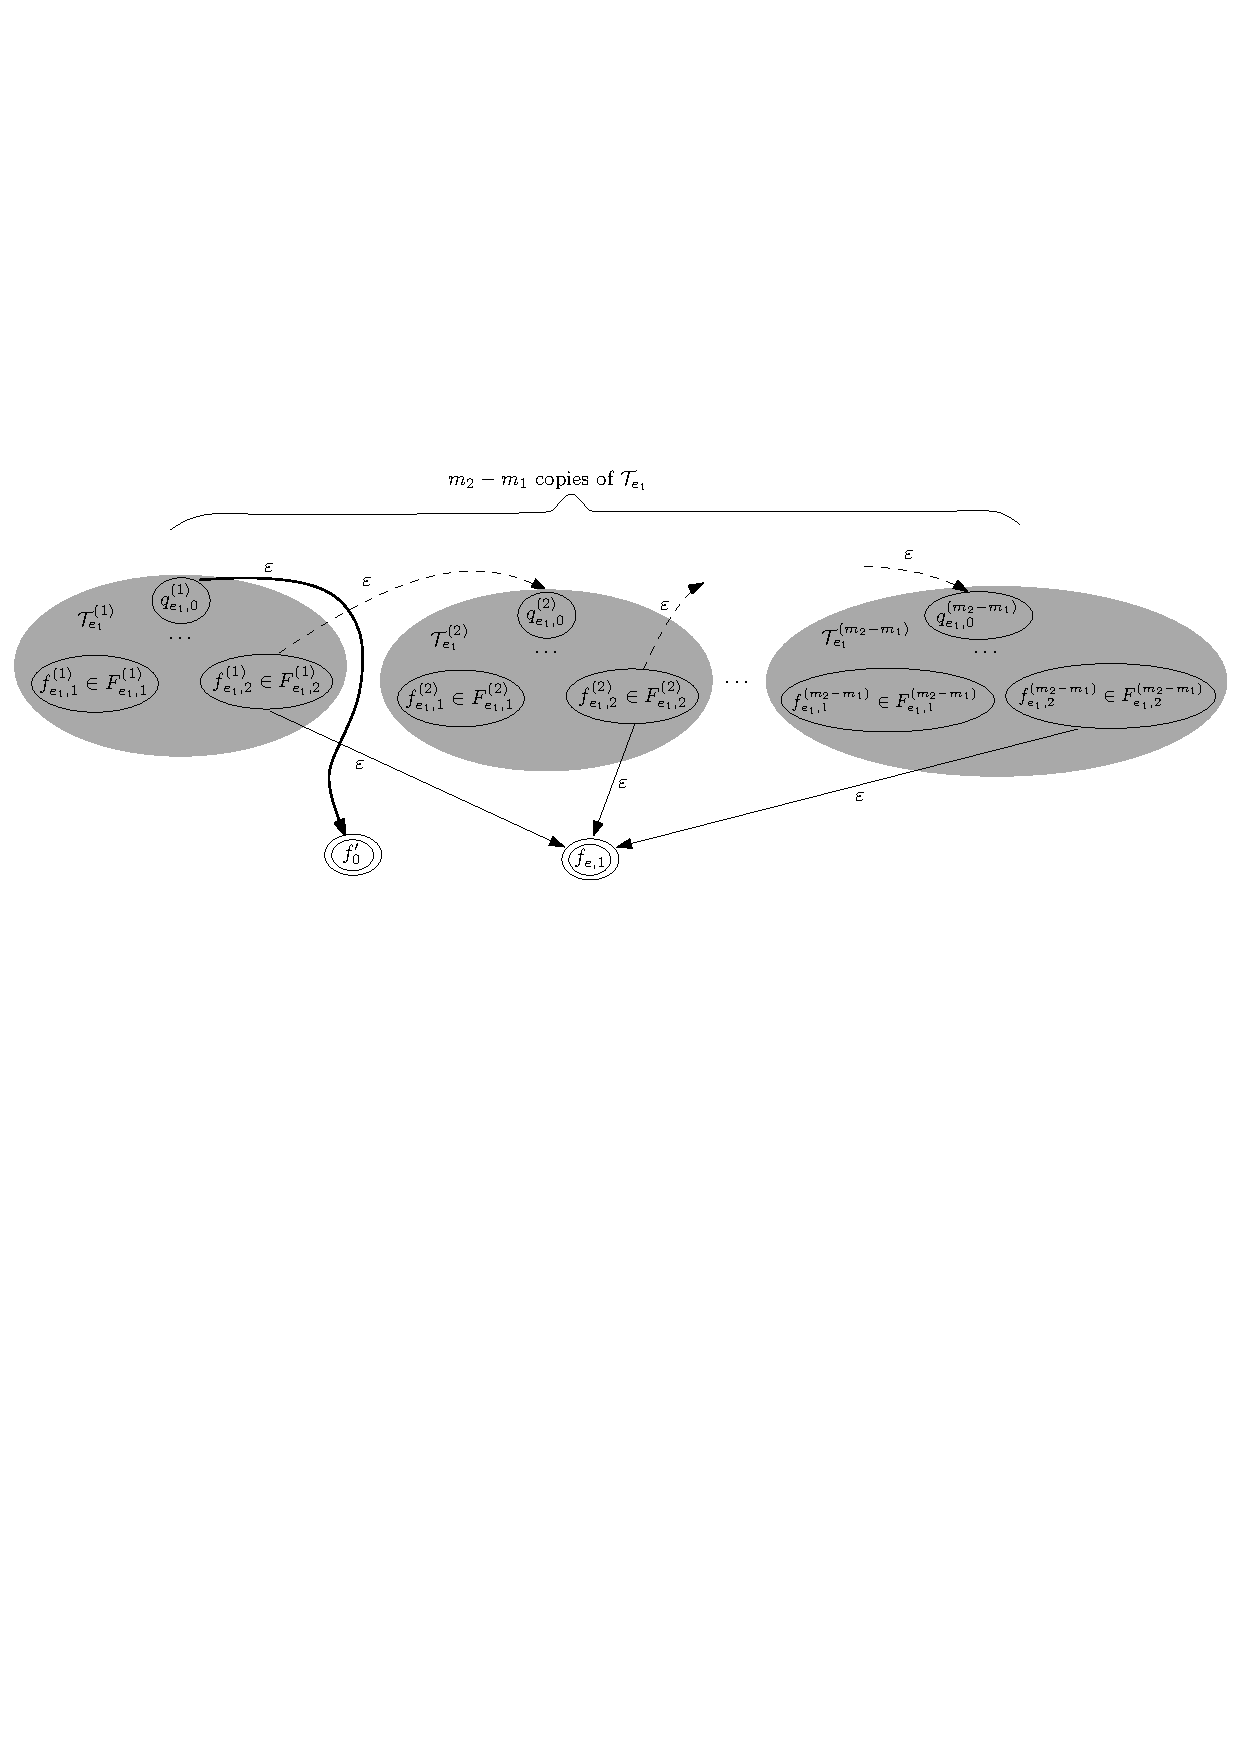
\includegraphics[width = 0.8\textwidth]{reg2pfa-5.pdf}
%			\caption{The PSST $\cT^{\{1,m_2-m_1\}?}_{e_1}$}
%			\label{fig-reg2pfa-5}
%		\end{figure}  
%%%%%%%%%%%%%%%%%%%%%%%%%%%%%%%%%%%%%%%%%move to appendix %%%%%%%%%%%%%%%%%%%%%%%%%%%%%%%%%%%%%%%%%%%%%%%%%%%%%%%%%%%%%%%

 %can be constructed 
%(in linear time)

% such that 
%	\begin{itemize}
%		\item $\cA_e$ has a unique initial state without incoming transitions and a unique final state without outgoing transitions,
%		%
%		\item for subexpression $e'$ of $e$, $\cA_e$ contains at least one isomorphic copy of $\cA_{e'}$ (i.e. the PFA constructed for $e'$), denoted by ${\sf Sub}_{e'}[\cA_e]$. 
%	\end{itemize}

%Let us use ${\sf Sub}_{e'}[\cA_e]$ to denote the isomorphic copy of $\cA_{e'}$ in $\cA_e$, as mentioned in Proposition~\ref{prop-rwre-to-pfa}.

%\begin{proof}
%	For any $e \in \cgexp$, a PFA $\cA_e$ is constructed recursively in the sequel. The constructed PFA $\cA_e$ satisfies that 
%	\begin{itemize}
%		\item it has a unique initial state without incoming transitions and each of its final states has no outgoing transitions,
%		\item all the transitions out of the initial state are $\varepsilon$-transitions, 
%		\item the set of final states is divided into two disjoint subsets $F_1, F_2$ such that for each $w \in \Sigma^*$ satisfying that $q_0 \xrightarrow[\cA_e]{w} q$ for some $q \in F_1$ (resp. $q \in F_2$), $w = \varepsilon$ (resp. $w \neq \varepsilon$).
%	\end{itemize}



\begin{example}\label{exmp-pfa}
Consider {\pcre} $e = [a^+]$. 
%	The PFA corresponding to the RWRE $e = [[([\Gamma^+])\concat .?] \concat ([\Gamma^*])]$ 
	%in Example~\ref{exmp-regex-match-tree}
	%
We first construct $\cT_{a}$ and $\cT^-_{a^*}$ (recall that $\cT^-_{a^*}$ is obtained from $\cT_{a^*}$ by removing the string variable $x_{[a^*]}$, see Figure~\ref{fig-pfa}).  Then we construct $\cT_{e}$ from $\cT_{a} \concat \cT^-_{a^*}$ by adding the initial state $q_{[a^+],0}$, the string variable $x_{[a^+]}$, as well as the assignments for $x_{[a^+]}$ (see Figure~\ref{fig-pfa}). Note here only one copy of $\cT^-_{a^*}$ is used in $\cT_{a} \concat \cT^-_{a^*}$, since $\varepsilon$ is not accepted by $\cT_{a}$.
 %
%illustrated in Fig.~\ref{fig-pfa}, where the dashed (resp. thicker solid) lines represent the $\varepsilon$-transitions of lower (resp. higher) priorities than non-$\varepsilon$ transitions (if there is any), and the doubly circled states are final states. For instance, $\delta(q_1, \ell) = (q_1)$ for every $\ell \in \{0, \dots, 9\}$, $\delta(q_1, .) = ()$, $\tau(q_1) = ((); (q_2))$. Since the $\varepsilon$-transition has lower priority than the $\ell$-transition at the state $q_1$, whenever the currently scanned letter is $\ell \in \{0,\cdots,9\}$ at $q_1$,  the PFA will choose to go to $q_1$ greedily, until there is no more $\ell  \in \{0,\cdots,9\}$. (In this case, it has to choose the $\epsilon$-transition and goes to $q_2$.)
	%
	\begin{figure}[tb]
%		\vspace{-2mm}
		\centering
		%\rule{\linewidth}{0cm}
		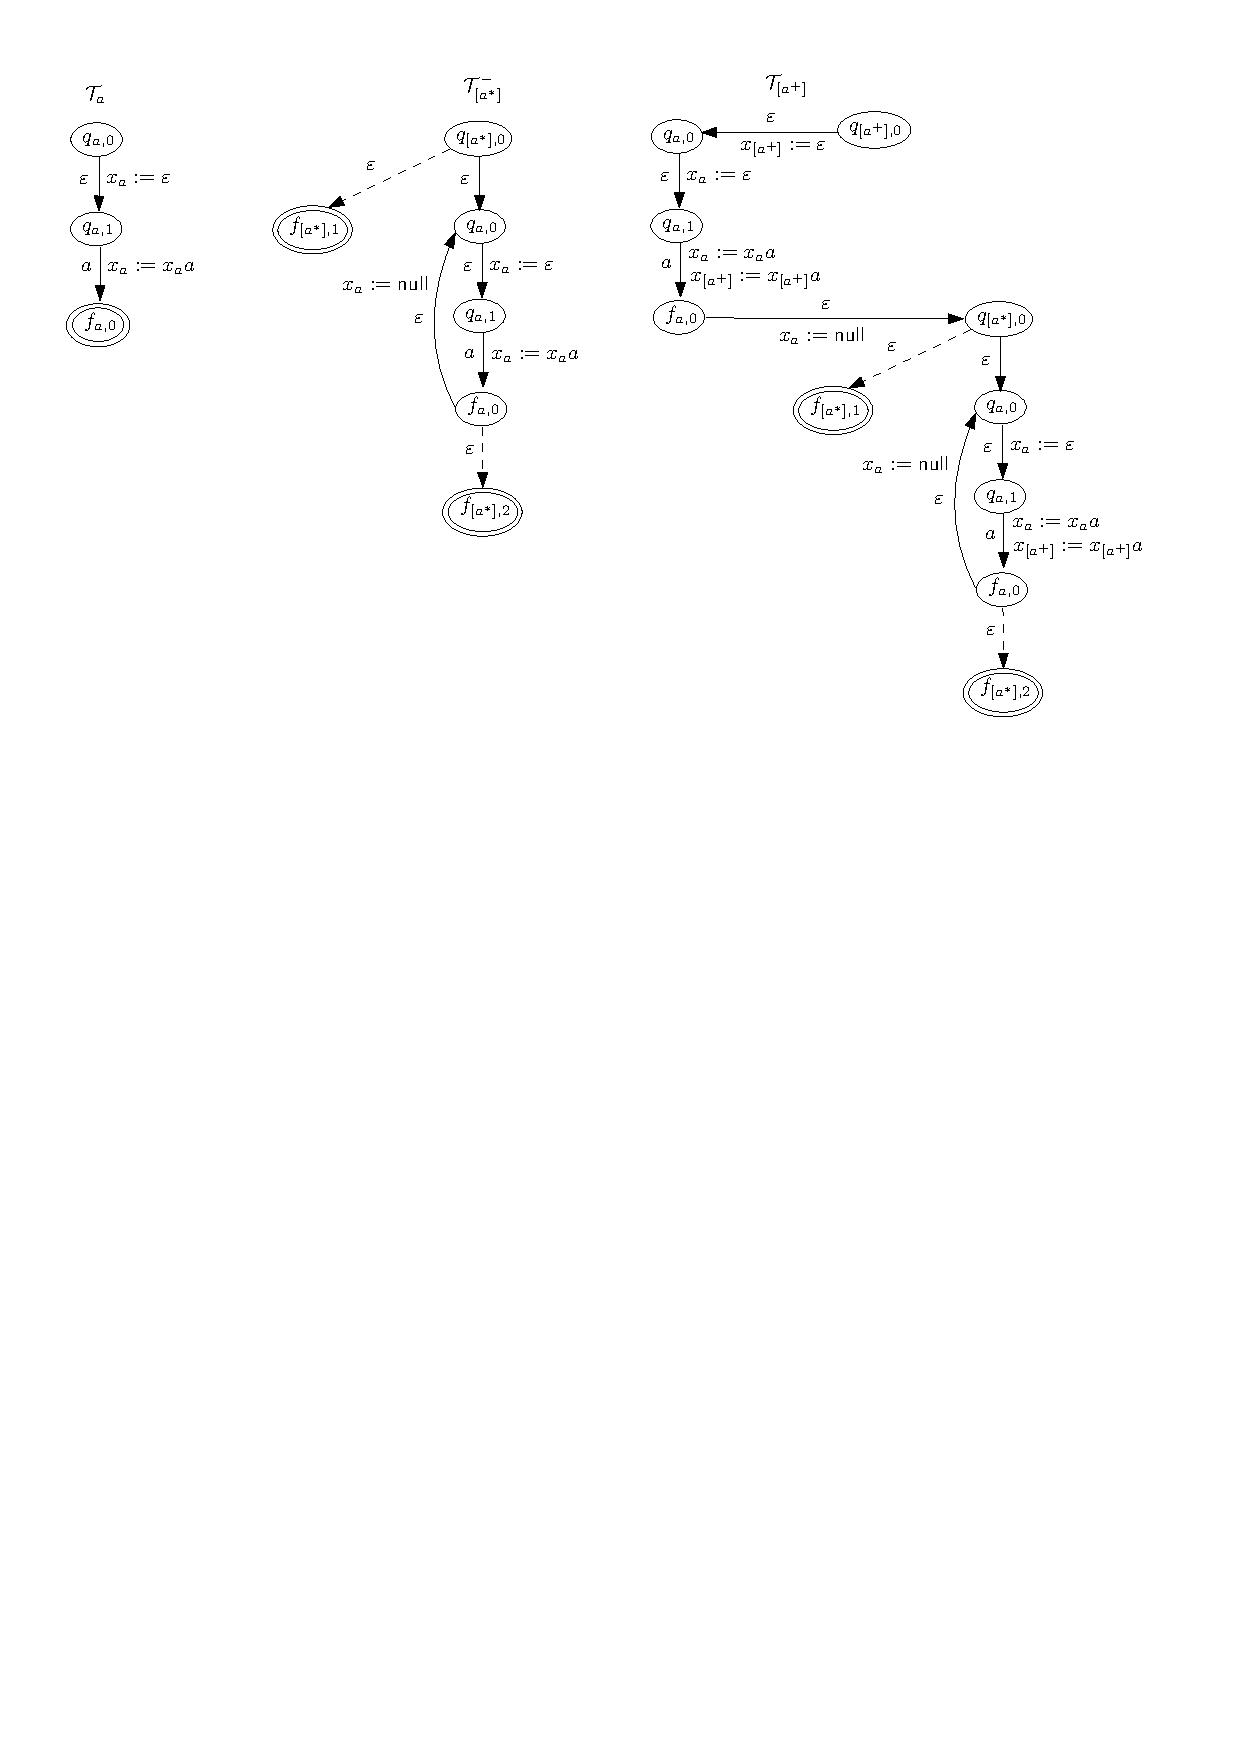
\includegraphics[width=0.9\textwidth]{pfa-new.pdf}
		\caption{The PSST $\cT_e$ for $e = [a^+]$}
		\label{fig-pfa}
		\vspace{-4mm}
	\end{figure}
\end{example}

